\documentclass[preprint,12pt,authoryear=false]{elsarticle}
\usepackage[utf8]{inputenc}
\usepackage[T1]{fontenc}
\usepackage{lmodern}
\usepackage{amsmath,amssymb}
\usepackage{graphicx}
\usepackage{booktabs}
\usepackage{tabularx}
\usepackage{multirow}
\usepackage{xcolor}
\usepackage{tikz}
\usetikzlibrary{positioning,arrows.meta,fit,backgrounds,calc}
\usepackage[hidelinks]{hyperref}
\usepackage{lineno}
\usepackage{siunitx}
\sisetup{detect-all}
\graphicspath{{figures/}}
\newcommand{\NumFaultTypes}{44}
\newcommand{\NumPoints}{1207}
\newcommand{\NumEquip}{54}
\newcommand{\NumSensorPts}{722}
\newcommand{\NumSoftPts}{325}
\newcommand{\NumTruthPts}{160}
\newcommand{\NumStdPts}{508}
\newcommand{\NumAdvPts}{244}
\newcommand{\NumNextPts}{295}
\newcommand{\NumModelPts}{269}
\newcommand{\NumCalcPts}{131}
\newcommand{\NumZonePts}{36}
\newcommand{\NumWxPts}{27}
\newcommand{\ValElecDiff}{+0.5}
\newcommand{\ValElecDiffAbs}{0.5}
\newcommand{\ValElecCV}{2.8}
\newcommand{\ValGasDiff}{5.2}
\newcommand{\ValGasDiffAbs}{5.2}
\newcommand{\ValClgDiffAbs}{1.3}
\newcommand{\ValFanDiffAbs}{0.2}
\newcommand{\ValZoneMAE}{0.03}
\newcommand{\ValWallVBAS}{300}
\newcommand{\ValWallVBASmin}{5.0}
\newcommand{\ValWallNative}{35}
\newcommand{\ValStepsPerSec}{351}
\newcommand{\DriftErr}{2.8}
\newcommand{\DriftFlow}{15}
\newcommand{\DriftHVAC}{4.2}
\newcommand{\FMoaGasW}{157}
\newcommand{\FMleakGasS}{16}
\newcommand{\FMleakComfS}{114}
\newcommand{\FMchwComfS}{1210}
\newcommand{\FMrhComfW}{162}
\newcommand{\FMchFoulS}{1.0}
\newcommand{\FMtwFoulS}{3.3}
\newcommand{\FMblFoulW}{55}
\newcommand{\FMschedS}{14.4}
\newcommand{\FddDetF}{0.74}
\newcommand{\FddDiagF}{0.24}
\newcommand{\FddTrainN}{8{,}064}
\newcommand{\FddTestN}{5{,}376}
\newcommand{\AiInj}{24}
\newcommand{\AiShIdeal}{5.2}
\newcommand{\AiShGasIdeal}{19}
\newcommand{\AiShSiteIdeal}{+2.8}
\newcommand{\AiSuIdeal}{0.5}
\newcommand{\AiShReal}{6.4}
\newcommand{\AiShGasReal}{21}
\newcommand{\AiShSiteReal}{+2.5}
\newcommand{\AiSuReal}{0.3}
\newcommand{\AiShBias}{3.3}
\newcommand{\AiShGasBias}{15}
\newcommand{\AiShSiteBias}{+3.0}
\newcommand{\AiSuBias}{0.1}
\newcommand{\SpeedMs}{3.3}
\newcommand{\SpeedMaxK}{92{,}000}
\newcommand{\SpeedErr}{0.00}
\newcommand{\NumHospitalPts}{3244}
\newcommand{\EnvPeakOut}{133}
\newcommand{\EnvPeakEight}{93}
\newcommand{\EnvHrsEight}{362}
\newcommand{\EnvPeakThirteen}{45}
\newcommand{\EnvHrsThirteen}{104}
\newcommand{\EnvPeakBypass}{111}
\newcommand{\EnvHrsBypass}{367}
\newcommand{\EnvPeakLock}{66}
\newcommand{\EnvHrsLock}{346}
\newcommand{\NumSensorClasses}{36}
\newcommand{\HospitalSps}{60}


\journal{Energy and Buildings}

\begin{document}
\begin{frontmatter}

\title{Virtual BAS: a physics-grounded, real-world-like building automation system emulator with labelled faults, sensor imperfections and stochastic operation for developing and testing building AI}

\author{Liang Zhang\corref{cor1}}
\ead{liangzhang1@arizona.edu}
\cortext[cor1]{Corresponding author.}
\affiliation{organization={University of Arizona},
            city={Tucson},
            state={AZ},
            country={USA}}

\begin{abstract}
Artificial intelligence for buildings, from fault detection and diagnosis to reinforcement-learning control and
\emph{ambient} or large-language-model operators, must work on the data of real building automation systems (BAS),
where sensors drift, readings go missing, occupants behave randomly and equipment fails. Real BAS data are scarce and
lack ground truth, while simulation test beds are usually idealised. This paper presents \emph{Virtual BAS}, an
open-source emulator that couples a step-wise EnergyPlus simulation (the \emph{inner space}, the physics) with a
labelled \emph{outer space} representing the real world: sensor and actuator models, BAS sequences that act only on
observed values, stochastic occupancy and events, and \NumFaultTypes{} fault and event types on five layers. A
local-loop emulation by set-point translation propagates sensor faults physically through loops solved inside
EnergyPlus. The clock runs from real time to more than \SpeedMaxK{} times real time, and humans and AI agents inject
faults at run time through a web GUI, a REST API, an MCP server and a Gymnasium interface. EnergyPlus models are
converted automatically; the DOE reference large office (\NumPoints{} points on \NumEquip{} pieces of equipment) is
the case study. Beyond typical BAS points, the point list covers the full indoor environment, an extended weather
station with forecasts, sub-meters and grid signals, each tagged as standard, advanced or next-generation
instrumentation. With ideal sensors, annual results match native EnergyPlus within \ValElecDiffAbs\% for electricity
and \ValGasDiffAbs\% for natural gas. Experiments demonstrate equipment-level fault impacts, labelled data for fault
detection (macro-F1 \FddDetF{}), AI agents in the loop, a wildfire-smoke episode that a standard BAS cannot observe,
and the conversion of five reference buildings. Eighteen uses are identified, spanning AI development, university
teaching, operator and facility-manager training, and the testing of commercial analytics products.
\end{abstract}

\begin{keyword}
Building automation system \sep EnergyPlus co-simulation \sep Fault injection \sep Sensor drift \sep Labelled dataset \sep
Fault detection and diagnosis \sep Reinforcement learning \sep Ambient AI \sep Digital twin \sep Large language model agents
\end{keyword}

\end{frontmatter}

\linenumbers

%==========================================================================================
\section{Introduction}
\label{sec:intro}

Commercial buildings are operated through building automation systems (BAS) that sample hundreds to thousands of
points---temperatures, flows, positions, powers, statuses---and execute control sequences on them. These data are the
substrate of almost every data-driven building application: automated fault detection and diagnosis (FDD)
\cite{katipamula2005review1,kim2018fddreview}, model predictive and reinforcement-learning (RL) control
\cite{wang2020rlreview,wei2017drl,zhang2018radiant}, and the recent wave of \emph{ambient AI} agents and large language
model (LLM) operators that are expected to monitor, explain and act on building operation continuously. The
development of such methods faces a persistent dilemma. Real BAS data are difficult to obtain, are proprietary and
building-specific, and above all have no ground truth: when a supply-air temperature reads 2~K above set point nobody
knows whether the coil, the valve, the controller or the sensor is at fault. Physics-based simulation provides
ground truth, but simulation test beds are usually \emph{idealised}: sensors are perfect, data are never missing, the
controller sees the true state and nothing breaks. Methods developed in such environments routinely fail when
transferred to real buildings, a gap that has been named as one of the central obstacles of RL in buildings
\cite{nweye2022realworld,dulacarnold2021challenges}.

Building simulation test beds have made large progress. BCVTB \cite{wetter2011bcvtb} enabled co-simulation of
EnergyPlus \cite{crawley2001energyplus} with external controllers; the Modelica Buildings library
\cite{wetter2014modelica} provides component-level dynamic models; BOPTEST \cite{blum2021boptest} defines
standardised emulators, key performance indicators and a REST interface for benchmarking control; the Advanced
Controls Test Bed \cite{marzullo2022actb}, Energym \cite{scharnhorst2021energym}, Sinergym \cite{jimenez2021sinergym}
and CityLearn \cite{vazquez2019citylearn} provide RL-oriented environments. For FDD, EnergyPlus has native fault models
\cite{zhang2017faults}, fault modelling has been reviewed comprehensively \cite{li2018faultreview}, and labelled
datasets with faulted and fault-free operation have been published \cite{wen2012rp1312,granderson2023dataset} together
with a unified fault taxonomy \cite{chen2021taxonomy}. What is still missing is an environment that behaves like a
\emph{real BAS as experienced by an AI}: one that (i) exposes the equipment-level point list of an actual BAS rather
than a reduced observation vector, (ii) places a \emph{real-world layer} between physics and observation in which
sensor drift, noise, data loss and random occupancy are present by default, (iii) lets the BAS controllers act on the
wrong values so that the physical consequences of imperfection are simulated rather than added afterwards, (iv)
allows anyone---a person, a script, or an AI agent---to inject abnormal conditions \emph{while the building runs}, at
a controllable pace from real time to as fast as possible, and (v) labels everything with mathematically defined
ground truth. The datasets cited above are static, and the control test beds are designed to benchmark controllers in
idealised, fixed scenarios; to the author's knowledge none combines these five properties. A sixth requirement follows
from field evidence on what BAS actually measure. In 90 buildings with semantic metadata, temperature streams
outnumbered power meters by two orders of magnitude, and only 8\% of the buildings had the points needed to compute an
energy-use intensity \cite{fierro2019mortar}; installed CO$_2$ sensors had mean absolute errors of 118--138~ppm
\cite{fisk2010co2}. Indoor environmental quality beyond temperature, humidity and CO$_2$ \cite{wellv2}, occupant
counts and feedback, coil energy meters, actuator feedback and grid signals are rarely available. An emulator should
therefore (vi) expose both the instrumentation of today's BAS and the next-generation points that AI applications
need, so that the value of additional sensing can be quantified against ground truth.

The same gap affects people as much as algorithms. Operational problems are pervasive and costly: commissioning of
existing buildings, i.e. finding and fixing such problems, yielded a median whole-building energy saving of 16\% in a
compilation of 643 buildings \cite{mills2011commissioning}, and correctly implemented and tuned controls, accurate
sensors and fault correction could save about 29\% of the energy of US commercial buildings
\cite{fernandez2017controls}. Capturing these savings depends on operators, facility managers, technicians and
commissioning agents who can read a BAS and diagnose what it shows. They learn mostly on live buildings, where faults
cannot be staged on demand, the true state is unknown, and mistakes affect occupants and equipment. Aviation and
nuclear power train and examine their operators on full-scope simulators governed by standards \cite{ans35}, and
autonomous driving develops and validates its AI in open simulators before it reaches the road
\cite{dosovitskiy2017carla}. Building operation has only a few research prototypes of this kind, such as a hybrid
simulator connected to a real controller for community-college training \cite{xu2004training} and a video game that
introduces a university HVAC-control course \cite{johra2020geenie}. Ambient AI and LLM operators
\cite{zhang2024llmbem,zhang2024llmcontrol}, which are meant to run continuously beside or instead of a human operator,
need such an environment even more: they must be trained, evaluated and stress-tested on realistic BAS behaviour before
they are allowed to act on a real building. A realistic, interactive and labelled virtual BAS is therefore a shared
infrastructure for AI research, education, workforce training and industry practice (Section~\ref{sec:uses}).

This paper introduces \emph{Virtual BAS}, an open-source framework that is built around a simple separation
(Fig.~\ref{fig:architecture}). The \emph{inner space} is an EnergyPlus model advanced step by step through the
EnergyPlus Python API \cite{energyplusapi}; it represents the real physics. The \emph{outer space} is the real world
that surrounds the physics: sensors, actuators, the BAS software, occupants, weather perturbations, faults, operators
and AI agents. A canonical example motivates the design: if a zone temperature sensor drifts, the VAV controller does
not know it; it controls the drifting reading to set point, computes a wrong air-flow command and sends it to the
physical model, so the true zone temperature departs from comfort while the BAS screen shows everything in order. In
Virtual BAS this happens exactly so, and both trajectories and the defining equation of the drift are recorded.

The contributions are:
\begin{enumerate}
\item A formal inner/outer-space architecture for real-world-like BAS emulation, with mathematically defined sensor,
actuator, occupancy and fault models (\NumFaultTypes{} types on five layers) and a complete labelling scheme.
\item A \emph{local-loop emulation by set-point translation} that propagates sensor errors physically through control
loops that are solved inside EnergyPlus by ideal local controllers.
\item A generic \emph{BAS-ization} procedure that converts EnergyPlus models into BAS-ready emulators: topology
discovery, command binding, physical fault hooks, native control program extraction and semantic point list
generation (Project Haystack \cite{haystack} and Brick \cite{balaji2016brick}) with an availability tier for every
point (standard, advanced, next-generation).
\item An extended environment layer driven by EnergyPlus air flows and occupants---particle and VOC mass balances,
illuminance, sound, occupant feedback, weather forecasts and grid signals---that completes the indoor and outdoor
environment a BAS can observe.
\item An open-source implementation with a BAS-like web GUI, interactive time control (1$\times$ to as fast as
possible), BACnet-like priority overrides and five interfaces for humans and AI agents (GUI, scenario files, REST,
Model Context Protocol \cite{mcp2024}, Gymnasium \cite{towers2024gymnasium}).
\item A case study on the DOE reference large office \cite{deru2011reference} with eight experiments: verification
against native EnergyPlus, inner/outer coupling under sensor drift, an equipment-level fault impact matrix, labelled
data generation and an FDD benchmark, AI agents in the loop, indoor air quality under wildfire smoke, time-acceleration
accuracy, and generality across five reference buildings.
\item An analysis of eighteen uses of a virtual BAS across AI research, education and workforce training, industry
practice and the research community, each mapped to the features that enable it and to the evidence in this paper.
\end{enumerate}

The remainder is organised as follows. Section~\ref{sec:related} reviews related work. Section~\ref{sec:method}
presents the methodology. Section~\ref{sec:case} describes the case study and Section~\ref{sec:results} the
experiments. Section~\ref{sec:discussion} discusses potential uses and limitations, and Section~\ref{sec:conclusions}
concludes.

\begin{figure*}[t]
\centering
\resizebox{\textwidth}{!}{%
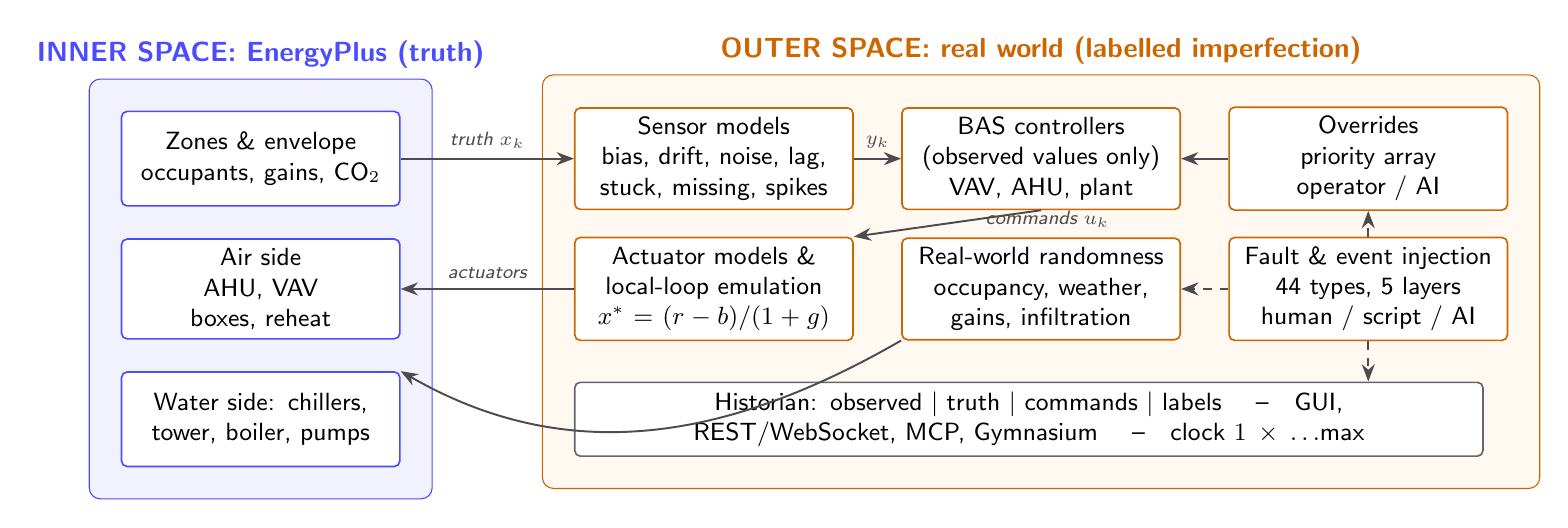
\begin{tikzpicture}[font=\sffamily\small, node distance=4mm and 6mm,
  blk/.style={draw, rounded corners=2pt, align=center, minimum height=12mm, text width=33mm, fill=white, line width=0.6pt},
  arr/.style={-{Stealth[length=2.2mm]}, line width=0.7pt, draw=black!70},
  lab/.style={font=\sffamily\scriptsize\itshape, text=black!70}]
\node[blk, draw=blue!70] (zone) {Zones \& envelope\\occupants, gains, CO$_2$};
\node[blk, draw=blue!70, below=of zone] (air) {Air side\\AHU, VAV boxes, reheat};
\node[blk, draw=blue!70, below=of air] (water) {Water side: chillers,\\tower, boiler, pumps};
\begin{scope}[on background layer]
\node[fit=(zone)(air)(water), draw=blue!70, fill=blue!5, rounded corners=4pt, inner sep=4mm, label={[font=\sffamily\bfseries, text=blue!70]above:INNER SPACE: EnergyPlus (truth)}] (inner) {};
\end{scope}
\node[blk, draw=orange!80!black, right=22mm of zone] (sens) {Sensor models\\bias, drift, noise, lag,\\stuck, missing, spikes};
\node[blk, draw=orange!80!black, right=of sens] (ctrl) {BAS controllers\\(observed values only)\\VAV, AHU, plant};
\node[blk, draw=orange!80!black, right=of ctrl] (ovr) {Overrides\\priority array\\operator / AI};
\node[blk, draw=orange!80!black, right=22mm of air] (act) {Actuator models \&\\local-loop emulation\\$x^*=(r-b)/(1+g)$};
\node[blk, draw=orange!80!black, right=of act] (rand) {Real-world randomness\\occupancy, weather,\\gains, infiltration};
\node[blk, draw=orange!80!black, right=of rand] (inj) {Fault \& event injection\\\NumFaultTypes{} types, 5 layers\\human / script / AI};
\node[blk, draw=black!60, right=22mm of water, text width=113mm, minimum height=9mm] (hist) {Historian: observed $\mid$ truth $\mid$ commands $\mid$ labels \quad--\quad GUI, REST/WebSocket, MCP, Gymnasium \quad--\quad clock $1\times\ldots$max};
\begin{scope}[on background layer]
\node[fit=(sens)(ovr)(inj)(hist), draw=orange!80!black, fill=orange!5, rounded corners=4pt, inner sep=4mm, label={[font=\sffamily\bfseries, text=orange!80!black]above:OUTER SPACE: real world (labelled imperfection)}] (outer) {};
\end{scope}
\draw[arr] (zone.east) -- node[lab, above]{truth $x_k$} (sens.west);
\draw[arr] (sens) -- node[lab, above]{$y_k$} (ctrl);
\draw[arr] (ovr) -- (ctrl);
\draw[arr] (ctrl.south) -- node[lab, right, pos=0.35]{commands $u_k$} (act.north east);
\draw[arr] (act.west) -- node[lab, above]{actuators} (air.east);
\draw[arr] (rand.south west) to[out=-150, in=-30] (water.north east);
\draw[arr, dashed] (inj.north) -- (ovr.south);
\draw[arr, dashed] (inj.west) -- (rand.east);
\draw[arr, dashed] (inj.south) -- (hist.north -| inj.south);
\end{tikzpicture}}
\caption{Inner/outer-space architecture of Virtual BAS. EnergyPlus (inner space) is advanced one BAS sample at a time;
the outer space measures it through imperfect sensors, controls it through BAS sequences that only see observed
values, and actuates it through actuator models. Faults and events modify sensors, controllers, actuators and the
EnergyPlus physics; everything is recorded with ground-truth labels.}
\label{fig:architecture}
\end{figure*}

%==========================================================================================
\section{Related work}
\label{sec:related}

\paragraph{Control test beds} Co-simulation of building models with external controllers dates back to BCVTB
\cite{wetter2011bcvtb}. BOPTEST \cite{blum2021boptest} standardised the evaluation of advanced control with
high-fidelity Modelica emulators \cite{wetter2014modelica}, a REST API, baseline controllers and key performance
indicators. The Advanced Controls Test Bed \cite{marzullo2022actb} connects Spawn-of-EnergyPlus models to Python
controllers through the BOPTEST and Alfalfa platforms. Energym \cite{scharnhorst2021energym}, Sinergym
\cite{jimenez2021sinergym} and CityLearn \cite{vazquez2019citylearn} provide Gym-style interfaces \cite{brockman2016gym}
for RL. These frameworks focus on \emph{benchmarking controllers} in reproducible conditions. They typically expose a
selected set of observations and control inputs, treat measurements as exact, and do not provide a library of
injectable sensor, actuator, control and network faults during operation. Reviews of RL for buildings
\cite{wang2020rlreview} and of real-world RL \cite{nweye2022realworld,dulacarnold2021challenges} emphasise exactly the
missing ingredients: partial and noisy observability, delays, safety constraints, non-stationarity and unexpected
events.

\paragraph{Fault modelling and FDD data} Fault modelling for HVAC has been reviewed in \cite{li2018faultreview}.
EnergyPlus supports a set of operational faults (sensor offsets, fouling of coils, chillers, boilers, towers and air
filters, thermostat offsets) \cite{zhang2017faults}. ASHRAE RP-1312 \cite{wen2012rp1312} and the LBNL dataset
\cite{granderson2023dataset} provide labelled faulted/fault-free data from simulation, laboratory and field, and a
unified taxonomy organises HVAC faults \cite{chen2021taxonomy}. These datasets are invaluable but \emph{static}: an
algorithm cannot interact with them, inject new faults, or close the loop. Classical FDD reviews
\cite{katipamula2005review1,kim2018fddreview} repeatedly identify the lack of ground-truth data and of test
environments with realistic sensor errors as a barrier to deployment.

\paragraph{Semantics and agents} Brick \cite{balaji2016brick} and Project Haystack \cite{haystack} provide semantic
models for BAS points, enabling portable analytics. LLM agents interacting with tools through the Model Context
Protocol \cite{mcp2024} create a new class of building applications whose evaluation requires an interactive,
semantically described BAS with ground truth.

\paragraph{Simulators for education and training} Full-scope training simulators are mandatory in nuclear power
\cite{ans35} and standard in aviation, and open simulators such as CARLA \cite{dosovitskiy2017carla} underpin the
development of autonomous-driving AI. In buildings, a hybrid simulator that connected a real-time HVAC simulation to a
real controller supported a community-college curriculum on control configuration and troubleshooting
\cite{xu2004training}, and a video game based on a building thermal model introduces a university course on HVAC
control \cite{johra2020geenie}. These tools teach control principles on simplified systems; none reproduces the point
list, graphics, alarms and failure modes of a commercial BAS on a full building with labelled faults.

\paragraph{Gap} Virtual BAS is complementary to the above: it reuses the physics of EnergyPlus and the standard
interfaces of RL environments, but its object of emulation is the \emph{BAS as a whole}---point list, controllers,
alarms, historian, operator overrides---embedded in a labelled real-world layer, interactive at any speed, open to fault
injection by humans and AI, and obtained automatically from existing EnergyPlus models.

%==========================================================================================
\section{Methodology}
\label{sec:method}

\subsection{Inner and outer space}

Let $\mathbf{x}_k$ be the physical state of the building at BAS sample $k$ as computed by EnergyPlus (the inner
space), $\mathbf{y}_k$ the values reported by the BAS, $\mathbf{u}_k$ the controller outputs and $\mathbf{a}_k$ the
values written to EnergyPlus actuators. With $\boldsymbol{\theta}(t)$ the parameters of the outer space, which are
modified by injections, one BAS sample is
\begin{align}
\mathbf{y}_k &= \mathcal{S}\big(\mathbf{x}_k;\boldsymbol{\theta}_S(t_k)\big), &
\mathbf{u}_k &= \mathcal{C}\big(\hat{\mathbf{y}}_{k};\boldsymbol{\theta}_C(t_k)\big), \label{eq:loop1}\\
\mathbf{a}_k &= \mathcal{A}\big(\mathbf{u}_k, \mathbf{x}_k;\boldsymbol{\theta}_A(t_k)\big), &
\mathbf{x}_{k+1} &= \mathcal{E}\big(\mathbf{x}_k,\mathbf{a}_k, \mathbf{w}_k;\boldsymbol{\theta}_E(t_k)\big), \label{eq:loop2}
\end{align}
where $\mathcal{S}$ is the sensor layer, $\hat{\mathbf{y}}_k$ the BAS present values (last valid sample of
$\mathbf{y}$), $\mathcal{C}$ the BAS control program, $\mathcal{A}$ the actuator layer including local-loop
emulation, $\mathcal{E}$ one EnergyPlus time step with weather and stochastic disturbances $\mathbf{w}_k$, and
$\boldsymbol{\theta}_E$ the physical fault parameters. The controller never sees $\mathbf{x}_k$. All quantities
$(\mathbf{x}_k,\mathbf{y}_k,\mathbf{u}_k,\boldsymbol{\theta}(t_k))$ are recorded.

\subsection{Step-wise co-simulation and time control}

EnergyPlus runs in a worker thread. At the beginning of every zone time step (callback \emph{begin system time step
before predictor}) the runner reads all output variables, meters and internal variables, calls the outer space and
writes the returned actuator values. Supervisory plant on/off overrides, which EnergyPlus clears during its HVAC
iterations, are re-applied in the \emph{inside system iteration loop} callback, and weather perturbations are applied
when EnergyPlus sets the current weather. EnergyPlus is suspended while the outer space computes, so the simulation is
truly stepped. Sizing and warm-up periods are excluded from the BAS time line. Values read at the start of step $k$
refer to the end of step $k-1$, which is the instant at which a BAS samples.

The pace is set by a speed factor $s$ (simulated seconds per wall-clock second). With BAS interval $\Delta t$ the
target wall-clock time of sample $k$ is $\tau_k = \tau_{k-1} + \Delta t / s$; the runner sleeps until $\tau_k$ in short
slices so that speed changes, pause and single-step requests issued through the GUI or API take effect immediately.
$s=\infty$ (``max'') runs as fast as possible.

\subsection{BAS-ization of an EnergyPlus model}
\label{sec:bas-ization}

A BAS-ready model is obtained from any EnergyPlus model by seven transformations (Table~\ref{tab:transformations}). The
HVAC topology is discovered from EnergyPlus' own connection objects (\texttt{AirLoopHVAC}, branches, supply paths,
zone splitters, \texttt{ZoneHVAC:EquipmentConnections}, plant and condenser loops), giving zones, terminal units, air
handling units with their outdoor-air system, coils and fan, and plant loops with chillers, boilers, towers and pumps.
Every quantity the BAS writes is bound to a dedicated \texttt{Schedule:Constant} (``command schedule''), e.g. a
\texttt{SetpointManager:Scheduled} on each AHU supply-air node and plant supply node, the fan availability schedule,
and the minimum-flow-fraction schedule of each VAV terminal (input method \emph{Scheduled}). Because the
minimum-flow input method changes EnergyPlus' autosizing of reheat coils, terminals and reheat coils are first
hard-sized with the values of a sizing run of the native configuration. Physical faults are hooked through EnergyPlus
\texttt{FaultModel:Fouling:*} objects whose availability and severity schedules are again command schedules. Finally,
the native schedules of fans, minimum outdoor air and thermostats are extracted so that the default BAS program
reproduces the native operation of the source model.

\begin{table}[!htbp]
\centering\small
\caption{Generic transformations of the BAS-ization procedure.}
\label{tab:transformations}
\begin{tabularx}{\linewidth}{lX}
\toprule
T1 & Simulation control: sizing performed, weather-file run period only \\
T2 & Zone time step $=$ BAS sampling interval (default 5 min) \\
T3 & Run period and calendar year \\
T4 & Remove file outputs (data are exchanged through the API) \\
T5 & Command binding: SAT, plant supply temperatures, fan enable, VAV air-flow commands $\rightarrow$ \texttt{Schedule:Constant}; terminals hard-sized from native sizing \\
T6 & Physical fault hooks: chiller, boiler and tower fouling models with command schedules \\
T7 & Zone CO$_2$ mass balance with actuatable outdoor concentration \\
\bottomrule
\end{tabularx}
\end{table}

From the topology a BAS point list is generated: for every piece of equipment the points a commercial BAS would
expose (Table~\ref{tab:points}), each with a stable identifier (\texttt{AHU-2/SA-T}), unit, kind (sensor, setpoint,
command, status, meter, virtual), sensor class, Project-Haystack style tags and a Brick class. Each sensor point is
bound to an EnergyPlus output variable, meter or derived expression (e.g. valve position as water flow over design
flow). Points that a BAS cannot measure but that are useful as labels (true occupant count, coil loads, COP, true
outdoor-air fraction, infiltration) are recorded as \emph{ground-truth-only} points. Duct static pressure, filter and
loop differential pressures, which EnergyPlus' fan and pump models do not resolve, are provided by documented
surrogate models, as are chiller refrigerant pressures (saturation temperatures from load- and fouling-dependent
approach temperatures and an R-134a vapour-pressure fit), boiler flue temperature and fan and pump vibration.

Every point carries an \emph{availability tier}. \emph{Standard} points are those of the ASHRAE Guideline~36 point
lists \cite{ashrae2021g36}, vendor chiller integrations and utility meters; \emph{advanced} points are found in
well-instrumented BAS (actuator position feedback, airflow and water-flow meters, sub-meters, refrigerant-side chiller
data, humidity and CO$_2$ in the return air); \emph{next-generation} points are rarely installed today but valuable for
analytics and AI (people counters, particle and VOC monitors, comfort stations, coil energy meters, vibration, weather
forecasts, tariff, grid carbon intensity and demand-response signals, occupant votes and complaints). BAS-calculated
points (run-hours, start counts, kW/ton, tower approach, 15-min demand, degree-days, outdoor-air fraction from the
mixing temperatures, Guideline~36 reset requests) are computed from \emph{observed} values, so sensor errors propagate
into them as in a real BAS. A scenario can restrict the exposed and recorded points to a set of tiers, e.g. to emulate
a typical BAS of today while keeping the full ground truth.

\begin{table}[!htbp]
\centering\footnotesize
\caption{BAS points generated for each equipment type (abbreviated); S = standard, A = advanced, N = next-generation tier.}
\label{tab:points}
\begin{tabularx}{\linewidth}{lX}
\toprule
Zone & \textbf{S}: ZN-T, ZN-CO2, ZN-OCC (PIR), heating/cooling set points, occupant set-point adjust; \textbf{A}: ZN-RH, ZN-DP, illuminance, lighting level, window contact, lighting power; \textbf{N}: people count, mean radiant and operative temperature, PMV, PPD, PM2.5, PM10, TVOC, sound level, occupant votes and hot/cold complaints, plug power; truth: occupants, daylight, infiltration, solar and internal gains \\
VAV box & \textbf{S}: DA-F, DA-F-SP, DA-T, DMPR-CMD, loop outputs, terminal mode, G36 requests, low-flow alarm; \textbf{A}: DMPR-POS, RHV-POS, velocity pressure; \textbf{N}: reheat-coil water flow and energy meter; truth: RH-Q \\
AHU & \textbf{S}: SA-T, SA-F, MA-T, RA-T, OA-T, OA-F, set points, OAD-CMD, ECON-EN, fan command/status/speed/Hz/power, DSP, FLT-DP, freeze-stat, smoke detector, run-hours, starts, calculated OA fraction; \textbf{A}: SA-RH, SA-DP, RA-RH, RA-CO2, OA-RH, coil leaving-air temperatures, valve/damper feedback, fan current; \textbf{N}: coil water temperatures, flows and energy meters, coil pressure drop, fan vibration; truth: CC-Q, OA fraction \\
Chiller & \textbf{S}: KW, STS, CHW/CDW entering and leaving temperatures, \%RLA, alarm, kW/ton, run-hours, starts; \textbf{A}: load, evaporator/condenser flows, refrigerant saturation temperatures and pressures; truth: PLR, COP \\
Boiler / tower / pump & \textbf{S}: STS, HW-LWT, HW-EWT, firing rate, alarm / fan power, status, speed, LWT, EWT, approach, range / KW, SPD, Hz, STS; \textbf{A}: load, gas, flow, flue temperature / make-up water; \textbf{N}: pump vibration \\
Plant loops & CHW-, HW-, CW-: ST, RT, F, DP, ST-SP, $\Delta T$; chilled-water tons and plant kW/ton \\
Weather & \textbf{S}: OA-T, OA-RH, degree-days; \textbf{A}: wet bulb, dew point, enthalpy, humidity ratio, pressure, wind speed and direction, global irradiance, outdoor illuminance, rain; \textbf{N}: direct and diffuse irradiance, sky cover and temperature, precipitation, outdoor PM2.5/PM10, 1/6/24-h forecasts \\
Meters, grid & \textbf{S}: building electricity and gas demand, water, totalisers, 15-min and peak demand; \textbf{A}: end-use sub-meters (HVAC, lighting, cooling, fans, pumps, heat rejection, heating, exterior lighting, DHW), tower make-up water; \textbf{N}: plug and elevator sub-meters, tariff, carbon intensity, demand-response event, cost and carbon today \\
\bottomrule
\end{tabularx}
\end{table}

\subsection{Sensor model}

For a physical quantity $x_k$ the recorded value is
\begin{align}
\tilde{x}_k &= \tilde{x}_{k-1} + \frac{\Delta t}{\tau+\Delta t}\left(x_k-\tilde{x}_{k-1}\right), \label{eq:lag}\\
d_k &= d_{k-1} + r\,\Delta t + \vartheta(\mu_d-d_{k-1})\,\Delta t + \sigma_d\sqrt{\Delta t}\,\xi_k, \label{eq:drift}\\
z_k &= (1+g)\,\tilde{x}_k + b + d_k + \sigma_n\varepsilon_k + B_k\sigma_s\eta_k, \label{eq:meas}\\
y_k &= \mathrm{clip}\!\left(\delta\,\mathrm{round}(z_k/\delta),\,y_{\min},\,y_{\max}\right), \label{eq:quant}
\end{align}
with first-order sensor dynamics (time constant $\tau$), drift composed of a linear rate $r$ and an
Ornstein--Uhlenbeck component \cite{uhlenbeck1930brownian}, installation gain error $g$ and bias $b$, white noise,
Bernoulli spikes $B_k\sim\mathrm{Bern}(p_s)$, quantisation $\delta$ and range limits. Two failure modes override the
output: a stuck sensor returns the value at the stuck instant, and a missing sample is \texttt{NaN}. Missing data
follow a two-state Gilbert--Elliott chain \cite{gilbert1960burst,elliott1963burst} with transition probabilities
$p_{gb}$ and $p_{bg}$, producing realistic bursts with stationary loss rate $p_{gb}/(p_{gb}+p_{bg})$. Binary sensors
(occupancy, status) use false-on/false-off probabilities. Installation parameters $(b,g,r)$ are drawn once per sensor
from data-sheet distributions of \NumSensorClasses{} sensor classes and scaled by a global \emph{realism} factor ($0$ = ideal sensors,
$1$ = typical commercial hardware). Each sensor uses an independent random stream, so that scenarios with different
faults share common random numbers. Fig.~\ref{fig:sensor} illustrates the model.

\begin{figure}[!htbp]
\centering
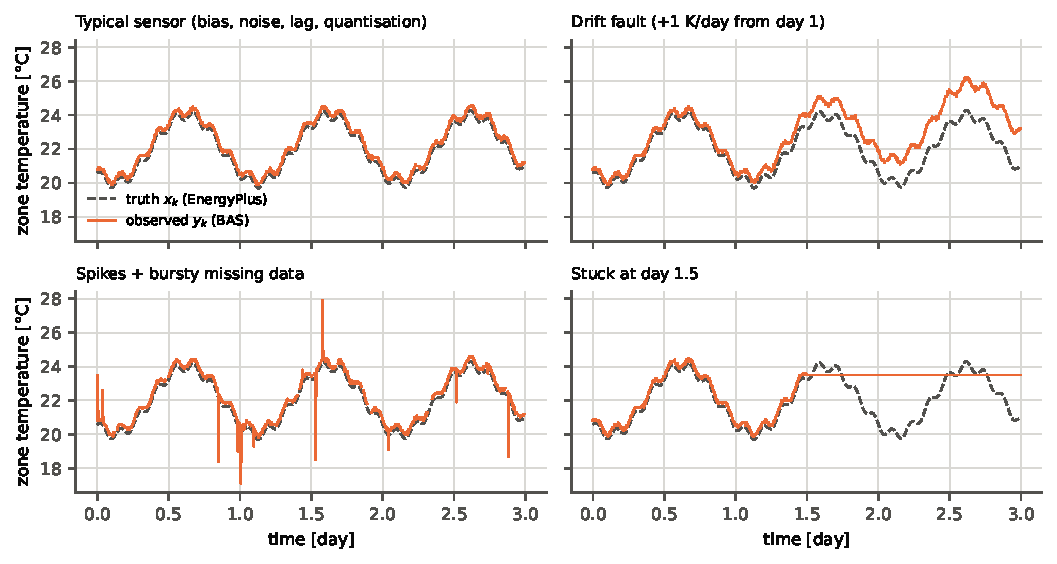
\includegraphics[width=\linewidth]{fig_sensor_model.pdf}
\caption{Sensor model output for a zone temperature sensor: typical commercial sensor, drift fault, spikes with bursty
missing data, and stuck sensor (dashed: EnergyPlus truth).}
\label{fig:sensor}
\end{figure}

\subsection{Actuators and local-loop emulation}

Explicit BAS outputs (VAV air-flow commands, outdoor-air damper position, fan start/stop) pass through actuator models
that can be stuck at a position, failed, or overridden. Some loops, however, are closed \emph{inside} EnergyPlus by
ideal local controllers: the reheat valve to the zone heating set point, the AHU coil valves to the supply-air set
point, chillers and boilers to their leaving water temperature, and the VAV box flow loop. A real local loop drives its
\emph{measured} value to the set point $r$. With the deterministic sensor map $y=(1+g)x+b$ (bias plus accumulated
drift), the steady state of a loop with integral action satisfies $(1+g)x^*+b=r$, hence
\begin{equation}
x^* = \frac{r-b}{1+g}. \label{eq:translation}
\end{equation}
Virtual BAS therefore hands $x^*$ instead of $r$ to the ideal EnergyPlus controller (\emph{set-point translation}).
If the reading is stuck or spoofed at value $v$, the integral action winds up and the actuator saturates:
$x^*=x_{\max}$ if $v<r$ and $x_{\min}$ otherwise for a direct process, and the opposite for a reverse (cooling)
process. If the reading is unavailable, the loop holds its last output. With Eq.~\eqref{eq:translation} every sensor
fault propagates physically, including through loops that the BAS does not compute explicitly.

The VAV terminals are controlled explicitly: the BAS computes an air-flow set point, the box flow loop is emulated
through Eq.~\eqref{eq:translation} applied to the air-flow sensor, and the resulting flow fraction is written to the
terminal's minimum-flow schedule while the EnergyPlus cooling set point of the zone is relaxed, so that EnergyPlus
delivers exactly the commanded flow. Reheat is supplied by the reheat local loop. The outdoor-air flow is written to
the \texttt{Controller:OutdoorAir} actuator as the commanded outdoor-air fraction times the sum of commanded box flows.

\subsection{Real-world randomness}

\paragraph{Occupancy} Each zone with $N$ design occupants follows the inhomogeneous Markov model of Page et al.
\cite{page2008occupancy}, driven by the zone's EnergyPlus occupancy schedule $P(t)$ scaled by a daily attendance factor
$a_d\sim\mathcal{U}(a_{\min},1)$:
\begin{gather}
T_{01}=\tfrac{\mu-1}{\mu+1}P_k+P_{k+1},\qquad
T_{11}=\tfrac{P_k-1}{P_k}\Big(\tfrac{\mu-1}{\mu+1}P_k+P_{k+1}\Big)+\tfrac{P_{k+1}}{P_k},\\
n_{k+1}=\mathrm{Bin}(n_k,T_{11})+\mathrm{Bin}(N-n_k,T_{01}),
\end{gather}
with mobility $\mu$. The count is written to the EnergyPlus \emph{People} actuator, so occupants affect heat gains and
CO$_2$; the BAS observes them only through PIR sensors with false-on/false-off rates (Fig.~\ref{fig:occupancy}).

\paragraph{Events} Weather perturbations (heat waves, cold snaps, cloud cover) are applied to the EnergyPlus weather
actuators as offsets/multipliers of the weather file; plug and lighting load changes, window opening (additional
infiltration), meetings, holidays and outdoor CO$_2$ changes complete the event library.

\subsection{Extended indoor and outdoor environment}
\label{sec:environment}

EnergyPlus solves the heat, moisture and CO$_2$ balances. Quantities that it does not model, but that occupants
experience and next-generation BAS measure, are computed in the outer space at every step from the EnergyPlus state,
so they remain consistent with the simulated air flows, occupants, lighting power and solar gains.

\paragraph{Particles and VOC} Each zone is a well-mixed volume $V$ supplied with $Q_s$ by its terminal and $Q_i$ by
infiltration:
\begin{align}
V\frac{dC}{dt} &= Q_s C_s + P\,Q_i C_o + S - (Q_s + Q_i + kV)\,C, \label{eq:iaq}\\
C_s &= (1-\eta)\left(x_{OA} C_o + (1-x_{OA})\,\bar C_{ret}\right), \nonumber
\end{align}
with outdoor concentration $C_o$, penetration factor $P$, deposition or sink rate $k$, indoor source $S$ (occupants,
materials, events), the AHU outdoor-air fraction $x_{OA}$ taken from EnergyPlus, filter efficiency $\eta$ by MERV class
\cite{ashrae522} and the flow-weighted return concentration $\bar C_{ret}$ of the zones served by the AHU.
Eq.~\eqref{eq:iaq} is integrated exactly over each step for PM2.5, the coarse fraction PM2.5--10 and TVOC (without
filtration). Outdoor PM2.5 follows a log-normal Ornstein--Uhlenbeck process with a diurnal traffic cycle;
\texttt{wildfire\_smoke}, \texttt{indoor\_pollutant\_source} and \texttt{filter\_bypass} injections act on $C_o$, $S$
and $\eta$.

\paragraph{Light and sound} Work-plane illuminance combines the lumen method for electric light and the daylight-flux
method, $E = E_d P_{light}/P_{light,d} + K_v U \Phi_{sol}/A$, with design illuminance $E_d$, luminous efficacy of
daylight $K_v$, utilisation factor $U$ and the solar flux $\Phi_{sol}$ transmitted by the zone's windows (EnergyPlus).
The background sound level is the energetic sum of terminal noise following the fan law
($L_{d} + 50\log_{10}(\dot V/\dot V_{max})$), speech scaled by the density of talking occupants, and a background floor.

\paragraph{Comfort and occupant feedback} Mean radiant and operative temperatures and the Fanger PMV and PPD
\cite{iso7730} come from EnergyPlus and are exposed as comfort-station points. Occupants submit thermal-sensation
votes $\mathrm{round}(\mathrm{PMV} + \sigma_i\varepsilon)$ through a feedback application at a Poisson rate, and file
hot or cold complaints at a rate proportional to $N\,\mathrm{PPD}$, split by a logistic function of PMV; votes and
complaint counts are BAS points.

\paragraph{Forecasts and grid} An hourly-issued 48-h weather forecast equals the weather file plus errors whose standard
deviation grows with lead time, $\sigma(h)=\sigma_0+\sigma_\infty(1-e^{-h/\tau})$, and that are AR(1)-correlated
between issues. The grid interface provides a time-of-use tariff, a synthetic marginal carbon intensity (diurnal
profile, solar dip and AR noise) and demand-response events with a requested shed; cost and carbon are accumulated as
KPIs. The forecast is also available as an API call and an MCP tool.

These models are deliberately simple, well documented and parameterised in the building configuration; they make the
corresponding points behave plausibly and causally, not reproduce a particular building.

\subsection{Faults and injections}

All abnormal or random conditions are \emph{injections} of a registered type. An injection has a target (point,
equipment, zone or building), start $t_0$, optional end $t_1$ and a severity profile
\begin{equation}
s(t)=\begin{cases}0 & t<t_0 \text{ or } t\ge t_1\\ 1 & \text{step}\\ \min\!\big(1,(t-t_0)/T_r\big) & \text{ramp (incipient)}\\
\mathbb{1}\!\left[((t-t_0)\bmod P)<D\,P\right] & \text{intermittent}\end{cases}
\end{equation}
that modulates one parameter, $\theta(t)=\theta_0+s(t)\,\Delta\theta$. Table~\ref{tab:faults} lists the library.
Equipment faults act inside EnergyPlus: fouling factors of chillers, boilers and towers through the native fault
models, filter loading through the fan pressure rise, fan degradation through the fan efficiency actuator, and trips
and stuck-closed valves through plant supervisory overrides. New types are registered with a decorator and immediately
appear in the GUI, the REST catalog and the MCP tools. A random fault generator draws arrivals from a Poisson process
with rate $\lambda$ per week and samples type, target, magnitude and duration from configurable distributions.

\begin{table*}[t]
\centering\footnotesize
\caption{Fault and event library (\NumFaultTypes{} types). Each type has a defining equation, typed parameters and a
target type; all are labelled with source (human, AI, scenario, random).}
\label{tab:faults}
\begin{tabularx}{\textwidth}{llX}
\toprule
Layer & Target & Types (parameter) \\
\midrule
Sensor & any sensor point & bias ($b$), drift ($r$, $d_{\max}$), gain ($g$), noise ($\sigma$), stuck, spikes ($p,\sigma_s$), dropout ($p$), override/spoofing ($v$) \\
Actuator & VAV, AHU & VAV damper stuck (position), reheat valve stuck closed/open, OA damper stuck, cooling/heating coil valve stuck closed, supply fan failure \\
Equipment & chiller, boiler, tower, AHU, pump & chiller/boiler/tower fouling (ratio $r$), filter fouling ($\Delta p$), fan degradation ($\ell$), equipment trip \\
Control & AHU, VAV, zone & schedule error (always on/off), PI mistuning (gain multiplier), economizer disabled/always on, SAT reset disabled, controller frozen, set-point override \\
Network & any equipment, historian & communication loss (controller off-line, BAS holds last values), historian outage \\
Events & zone, building & occupancy surge/vacancy, meeting, holiday, weather change ($\Delta T$, $\Delta\phi$, solar), window open (ACH), plug and lighting load change, outdoor CO$_2$ change \\
\bottomrule
\end{tabularx}
\end{table*}

\subsection{BAS control program}

The BAS control program acts on present values only and comprises: occupancy scheduling and night-cycle operation;
for each VAV box, cooling and heating PI loops on the zone temperature with air-flow set point between the minimum and
maximum flow (optional dual maximum); for each AHU, supply fan start/stop, supply-air temperature set point, duct static
pressure set point and an economizer with differential dry-bulb high limit, whose outdoor-air fraction combines a
mixing-equation feed-forward on observed return and outdoor temperatures with a PI trim on the mixed-air temperature
and a minimum outdoor-air limit computed from the sum of box air-flow set points; for the plant, chilled, hot and
condenser water supply temperature set points. PI controllers are discrete with anti-windup and are tuned for the
5-min sampling interval. Two profiles are provided: \emph{baseline}, which reproduces the native controls of the
source model (including its schedules) and is used for verification, and \emph{g36}, which implements trim-and-respond
resets of supply-air temperature, duct static pressure and chilled-water temperature and outdoor-air reset of hot-water
temperature inspired by ASHRAE Guideline 36 \cite{ashrae2021g36}. Any software point can be overridden through a
BACnet-like 16-level priority array (operator default priority 8, AI agents 10, BAS program 16). A rule-based alarm
engine raises alarms from observed values with on-delays, so that sensor faults can cause false alarms or mask real
ones.

\subsection{Labels and data products}

A run produces synchronised tables of observed values (the BAS trend log with gaps), truth, commands and per-sample
label bit masks (missing, stuck, spike, sensor fault active, communication loss, false binary reading, spoofed), a long
table of the severity of every active injection at every sample, the full injection definitions, sensor installation
parameters, alarm history and metadata (scenario, seed, realism, control configuration, EnergyPlus version). The exact
sensor error of every sample is $y_k-x_k$.

\subsection{Interfaces for humans and AI}

The web GUI (Fig.~\ref{fig:gui}) mimics a commercial BAS front end with building overview, AHU, VAV and plant graphics,
zone indoor-environment pages with a heat-map, a weather/forecast/grid/energy page, trends, alarms, a point explorer with priority overrides and an injection console generated from the fault catalog. A
global switch reveals the inner space (EnergyPlus truth) next to every observed value and highlights discrepancies.
The same functions are available through a REST/WebSocket API with OpenAPI documentation, a dependency-free Python
client, an MCP server exposing BAS tools (read points and trends, write set points, inspect the fault catalog, inject
and clear faults, control the clock) to LLM agents \cite{mcp2024}, and an in-process Gymnasium environment
\cite{towers2024gymnasium} whose agent writes set points at priority 10 and observes BAS values, with rewards computed
from the truth.

\begin{figure*}[t]
\centering
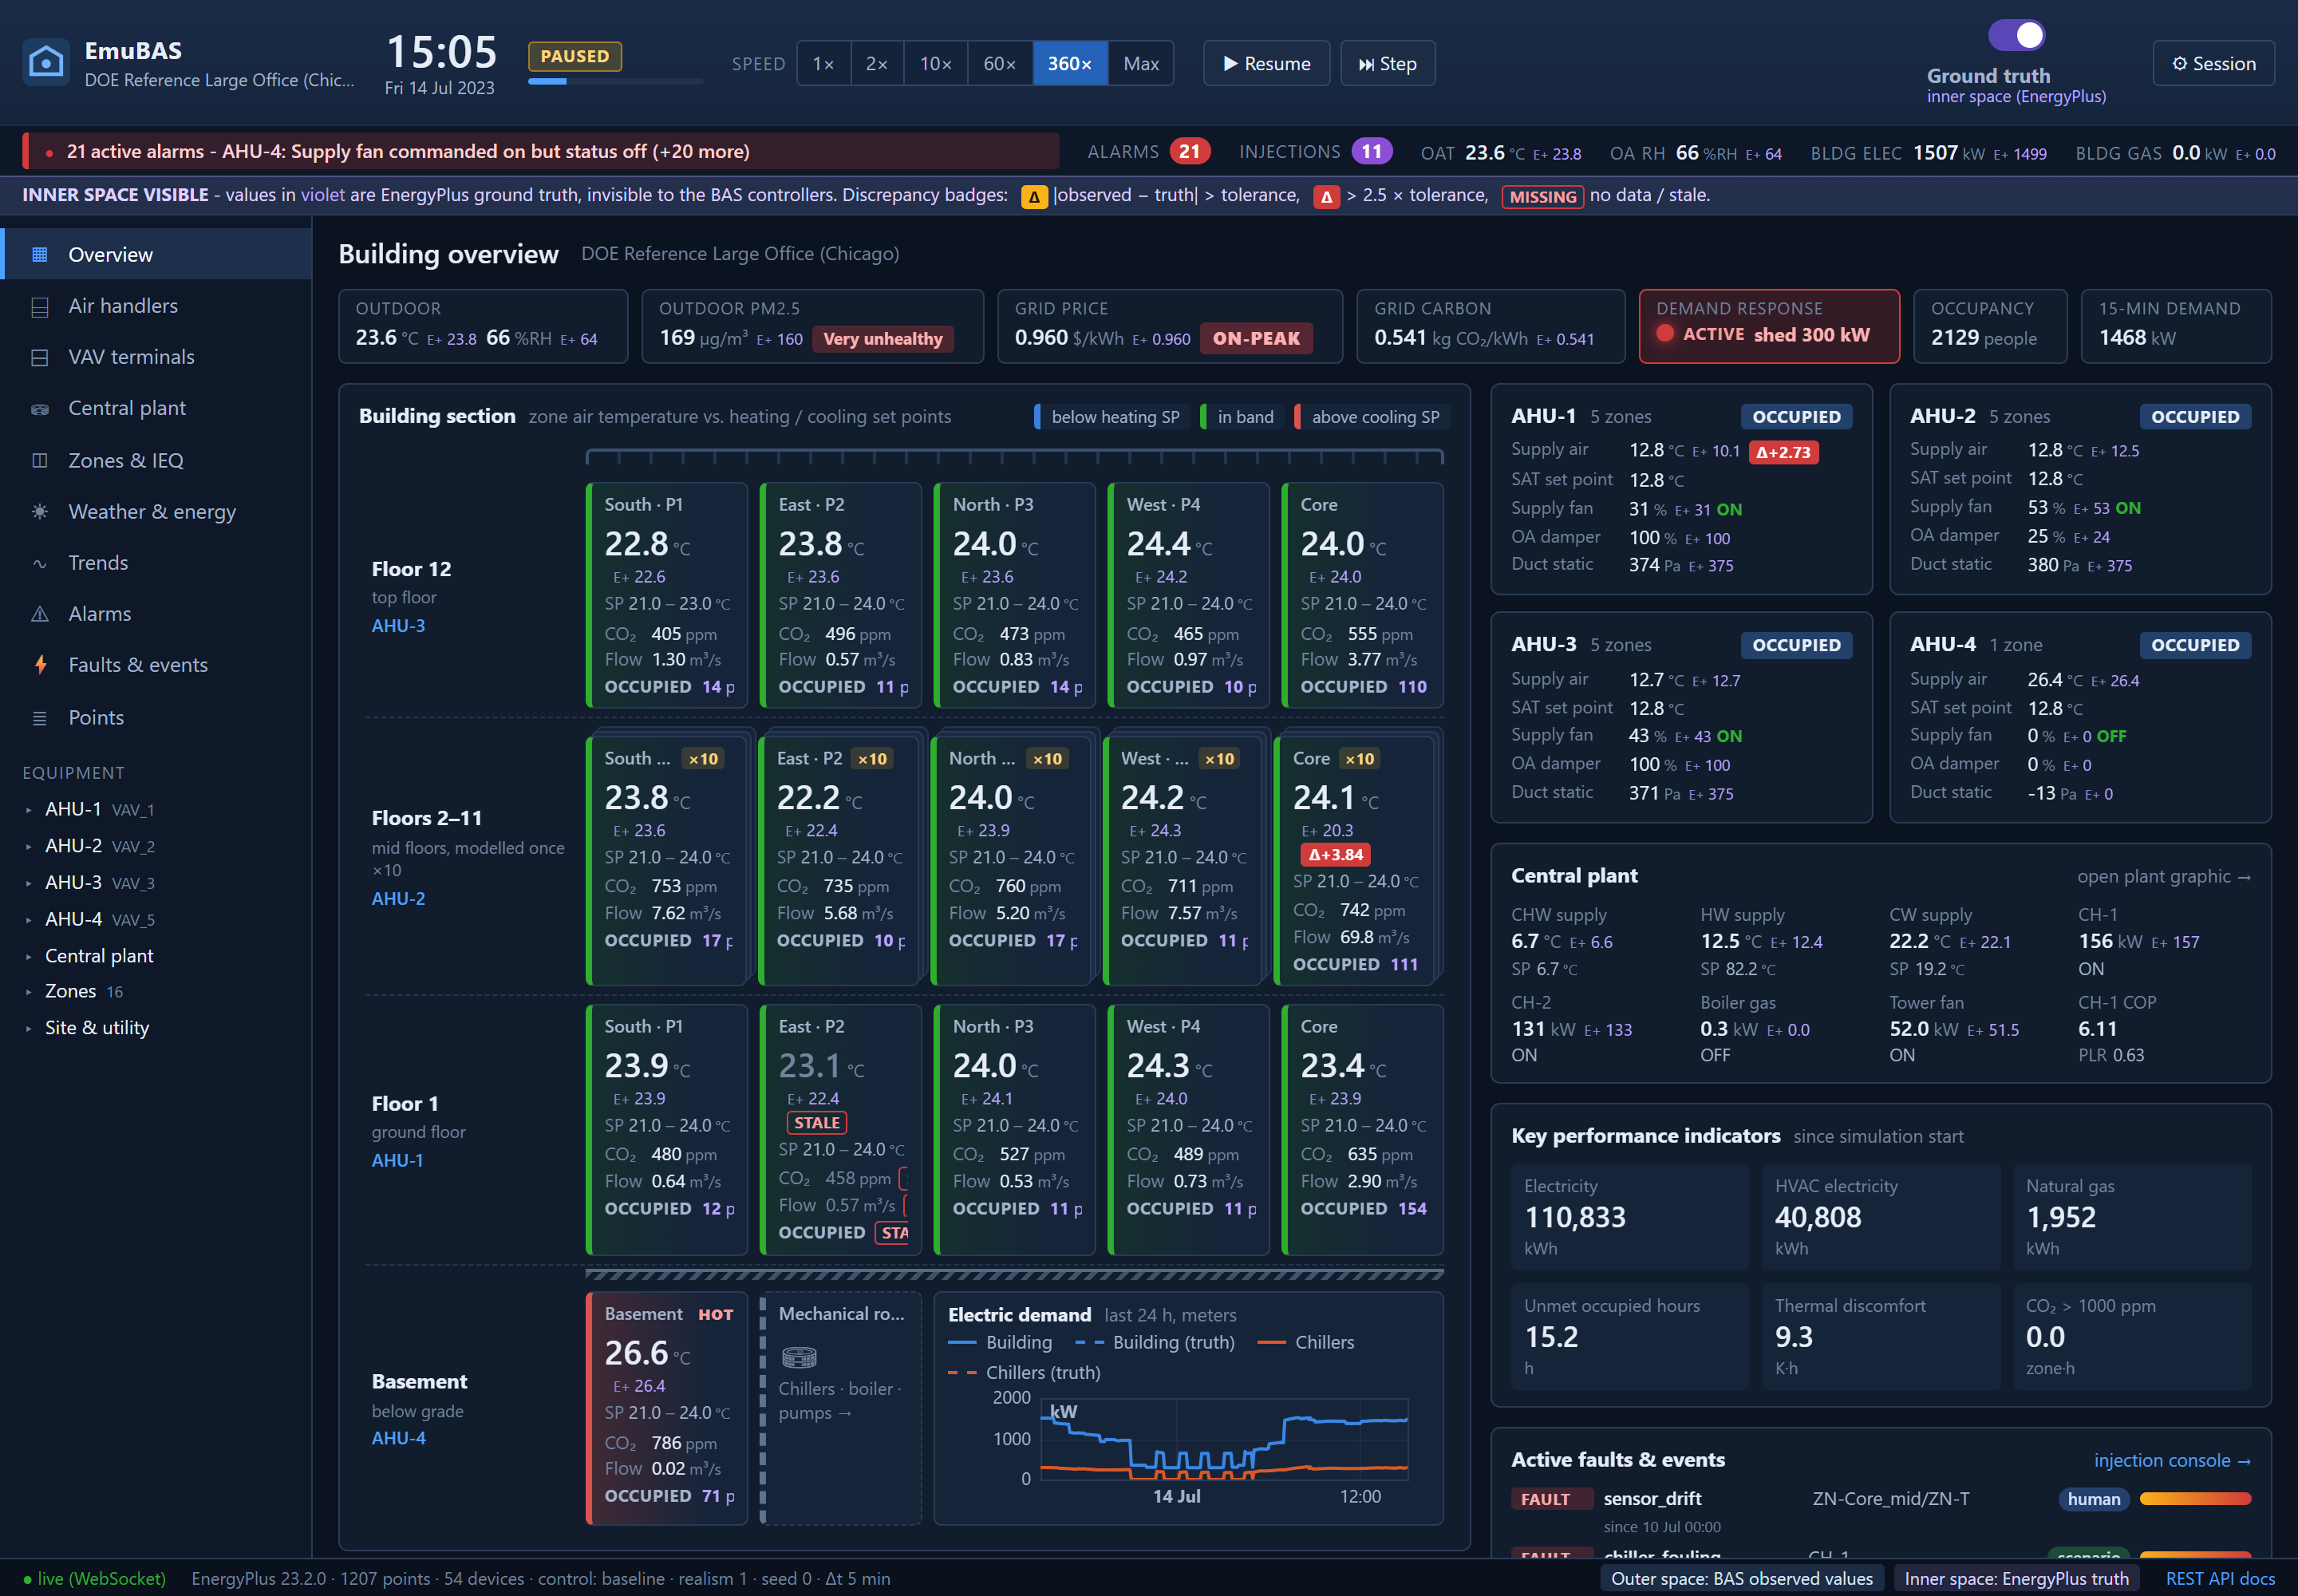
\includegraphics[width=0.49\textwidth]{gui_overview.png}\hfill
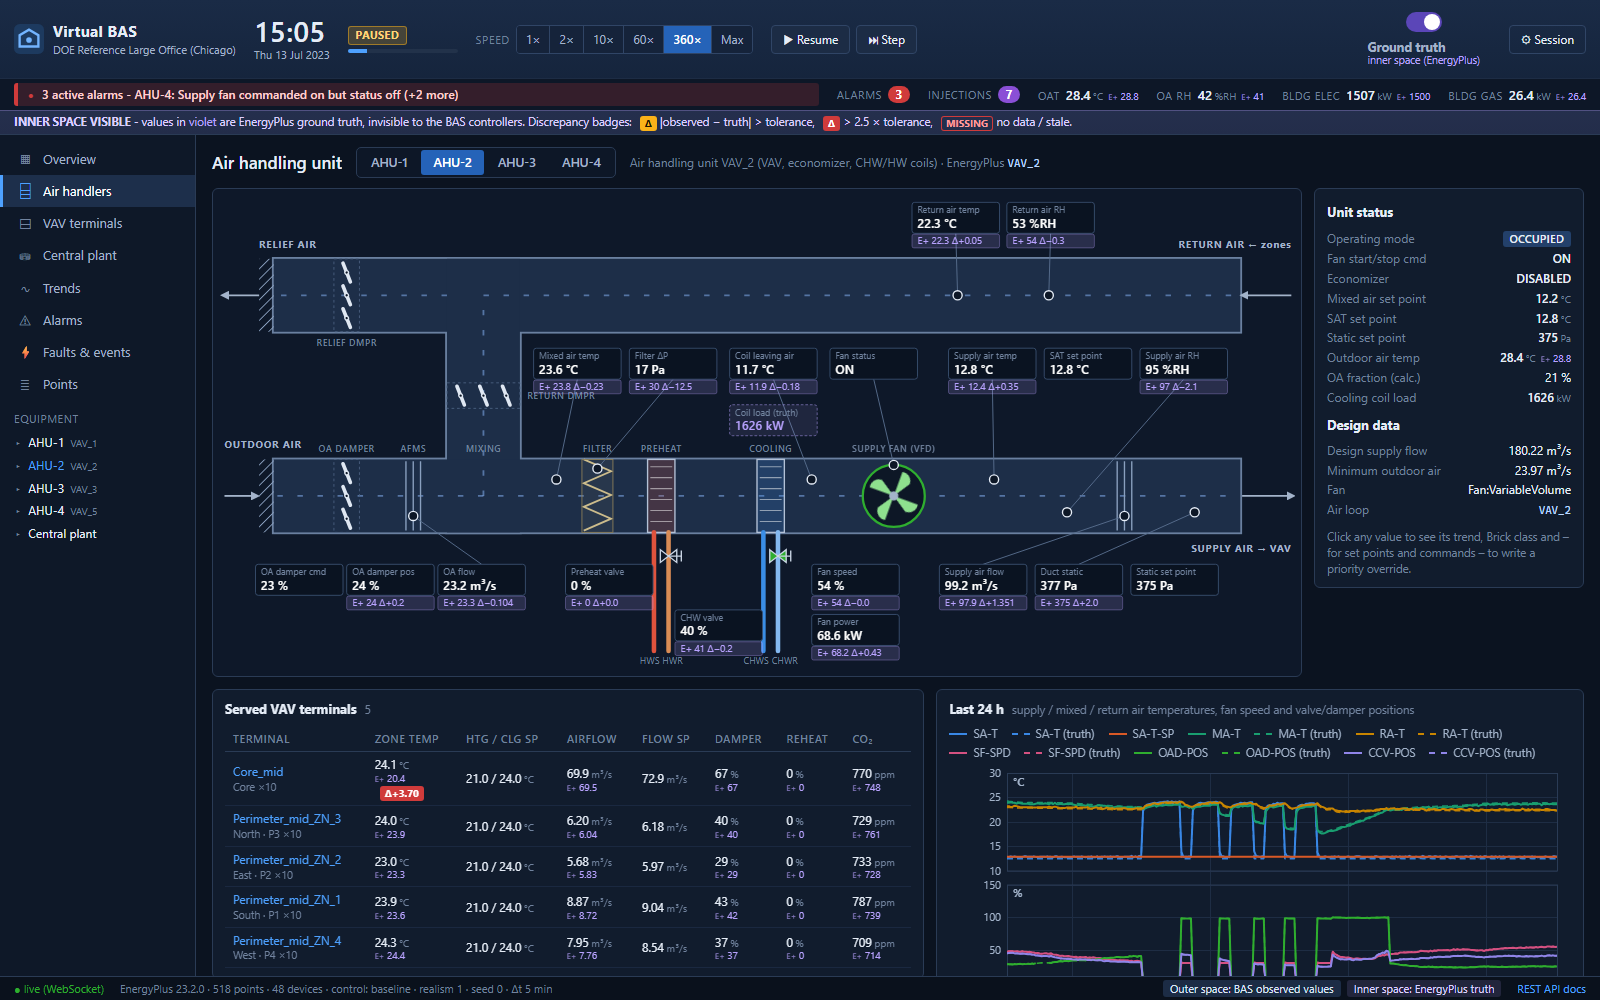
\includegraphics[width=0.49\textwidth]{gui_ahu.png}\\[2mm]
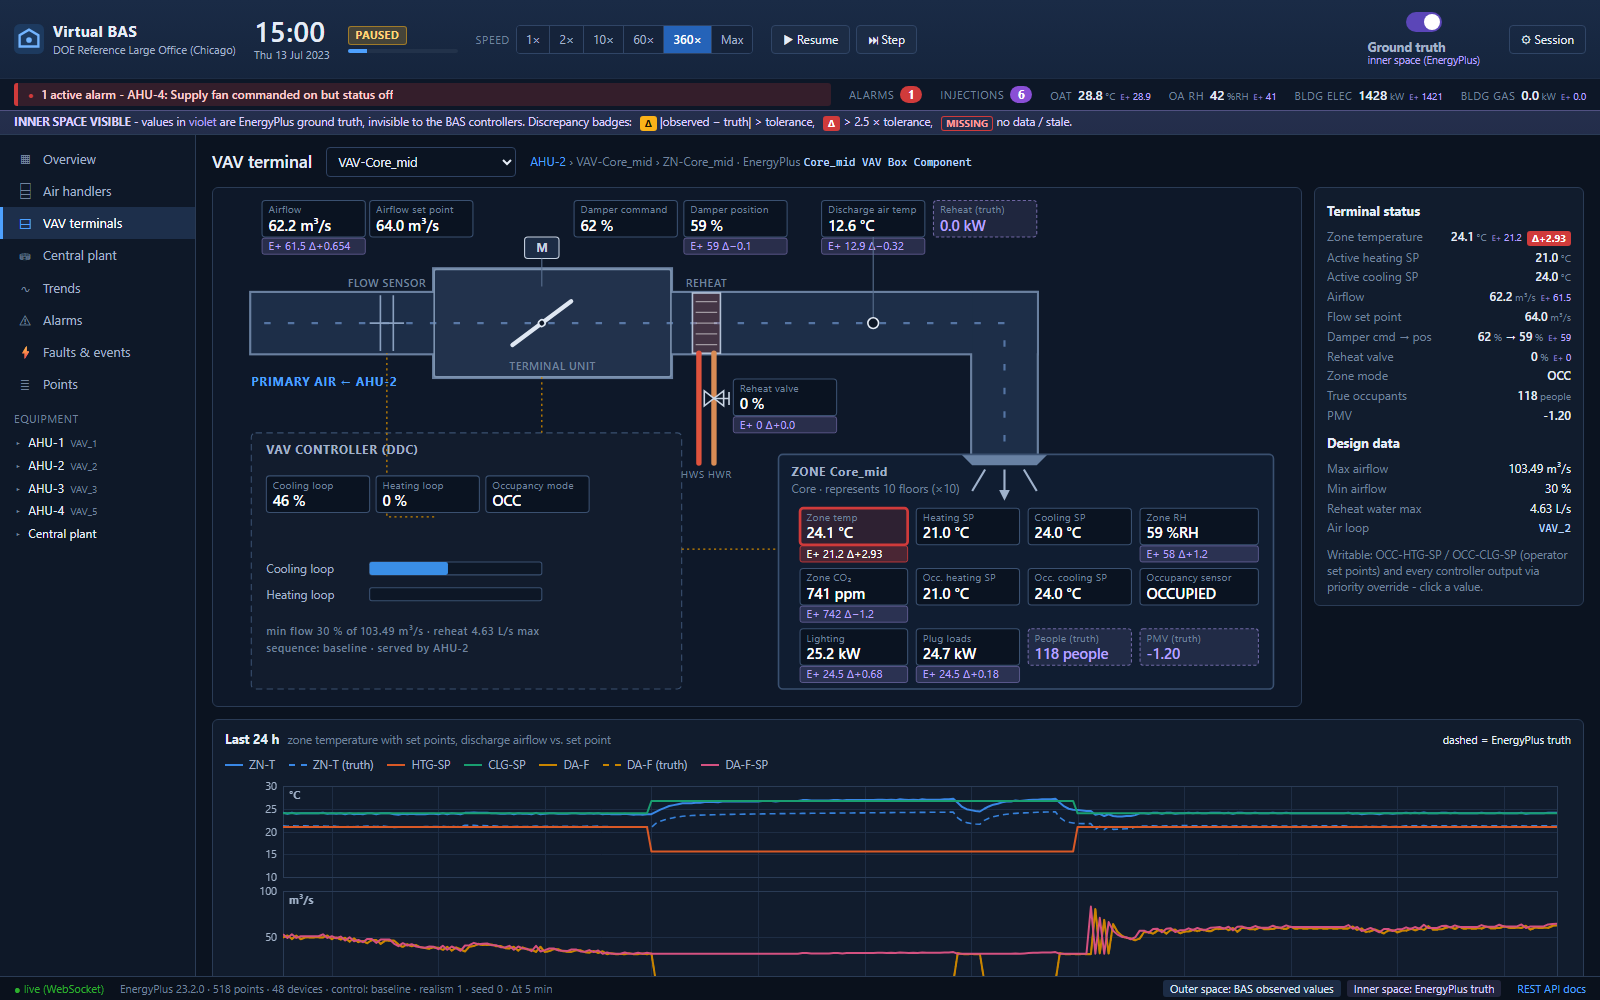
\includegraphics[width=0.49\textwidth]{gui_vav.png}\hfill
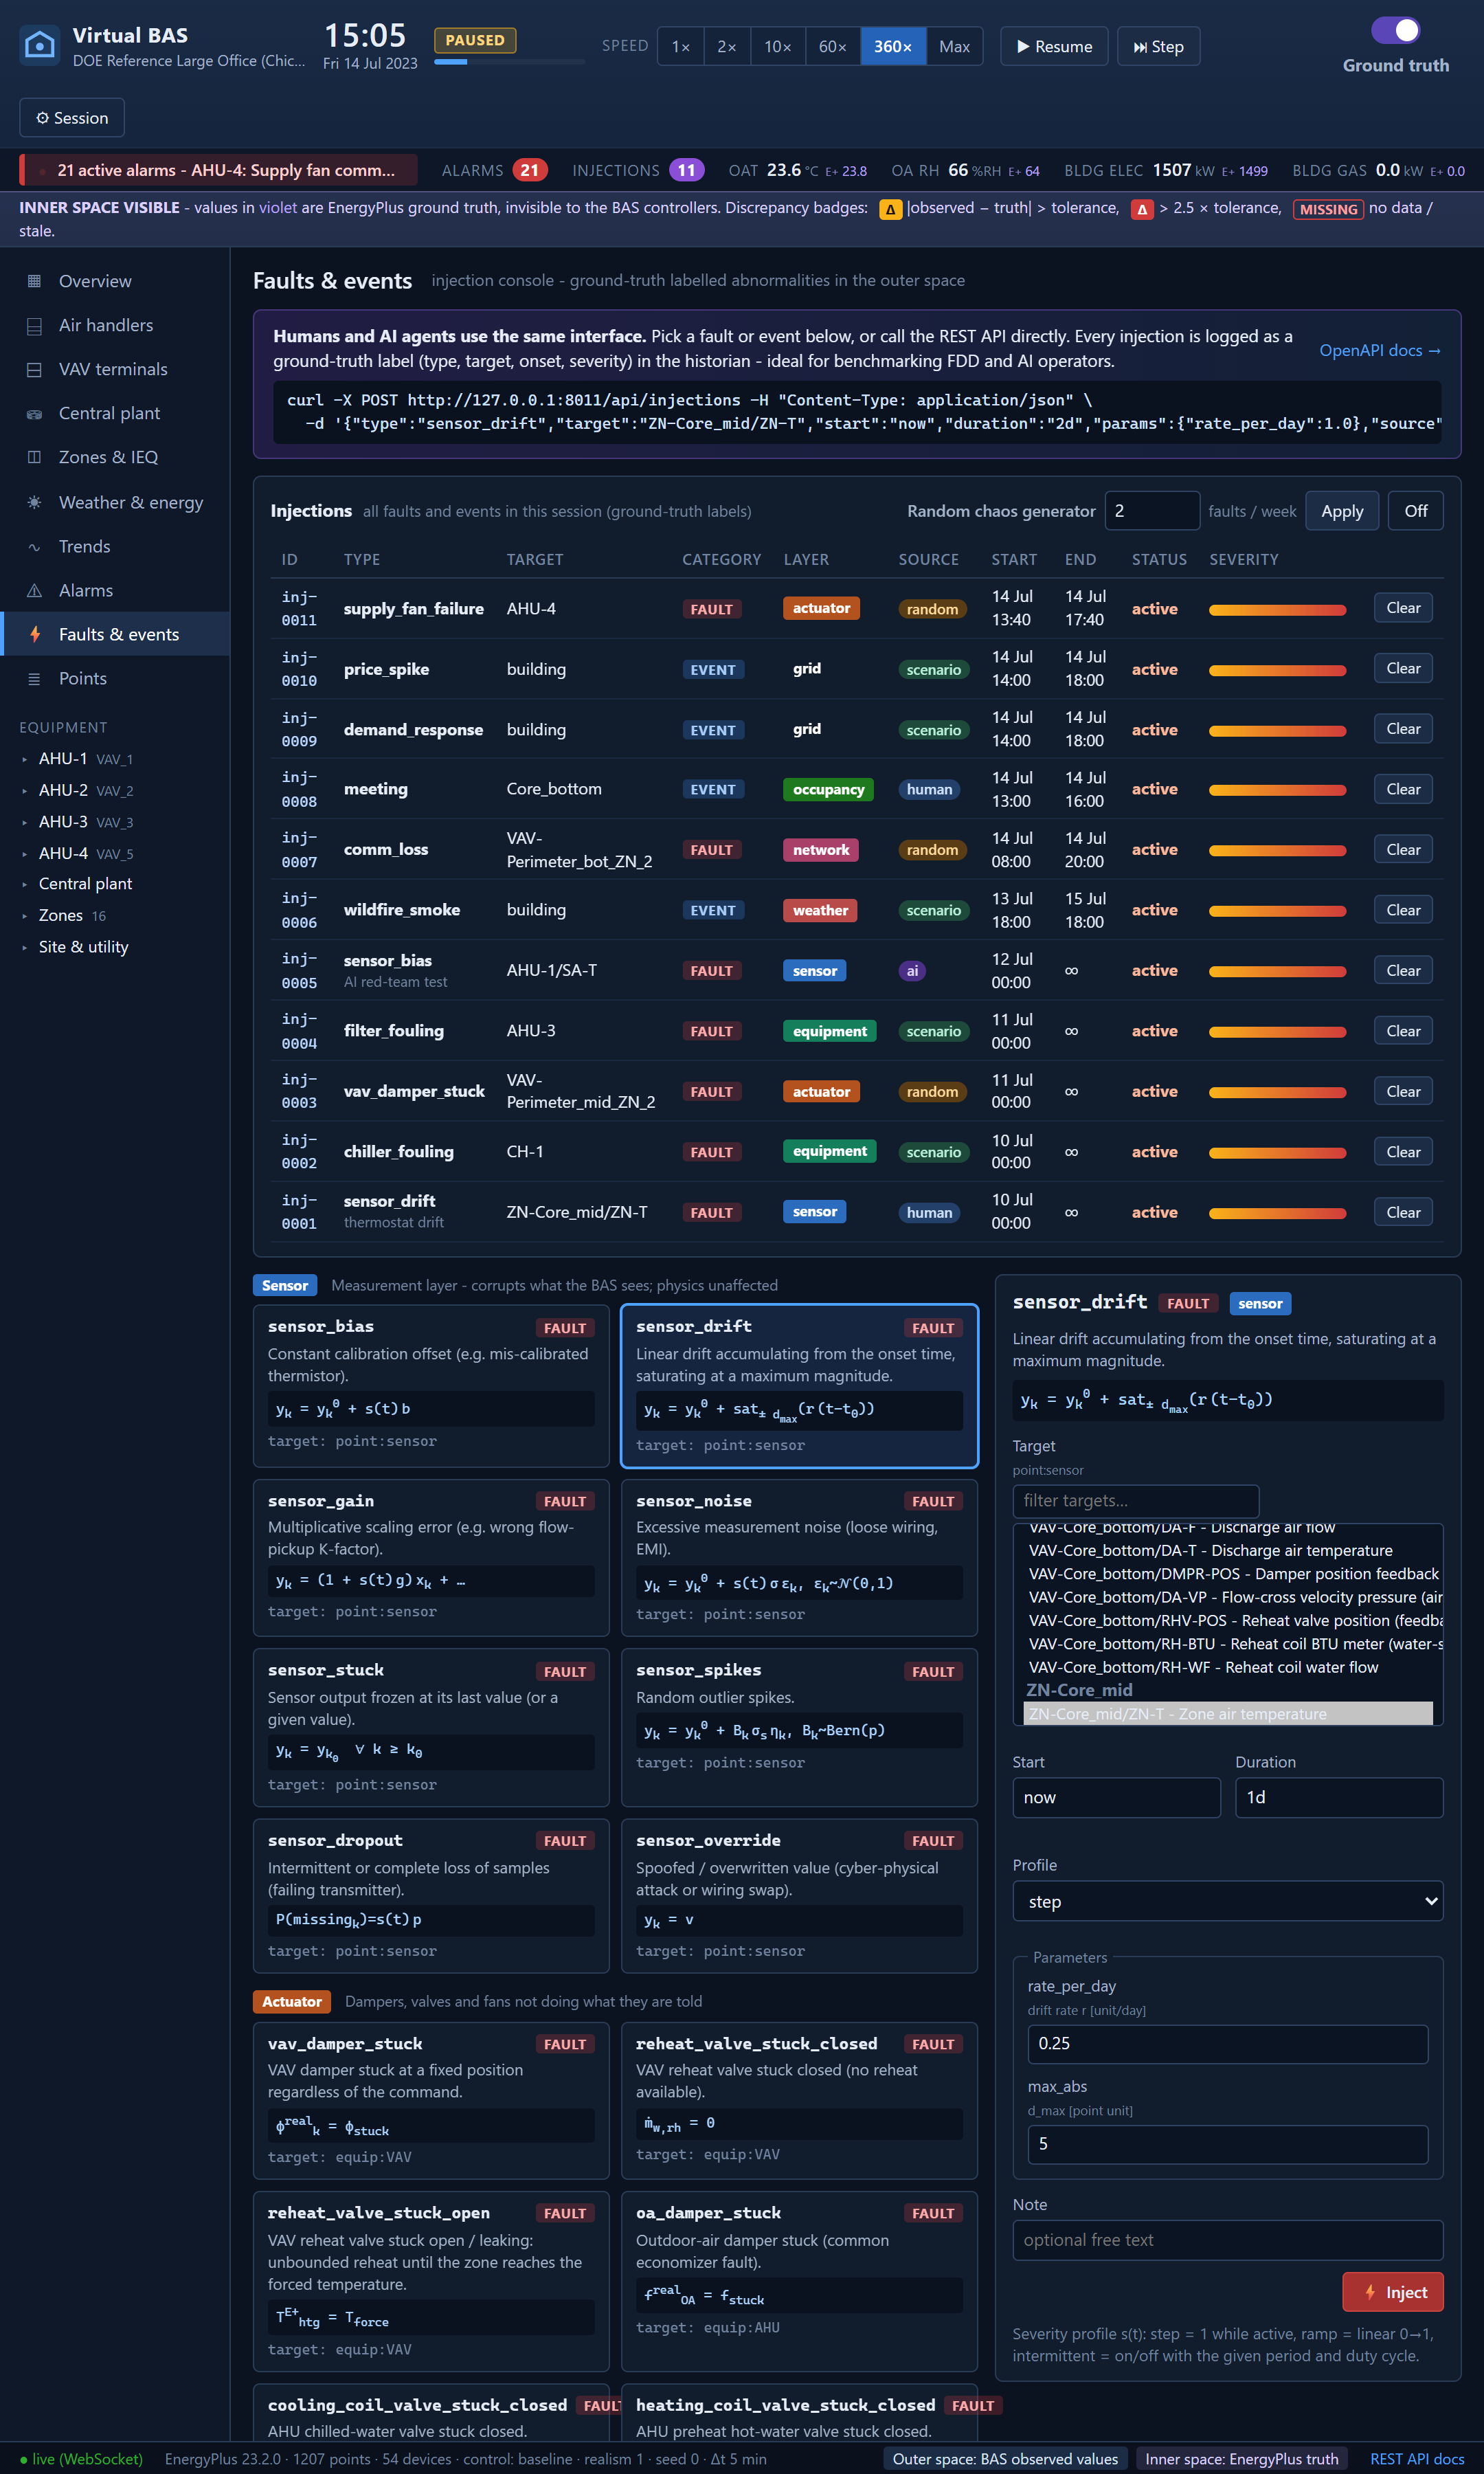
\includegraphics[width=0.49\textwidth]{gui_faults.png}\\[2mm]
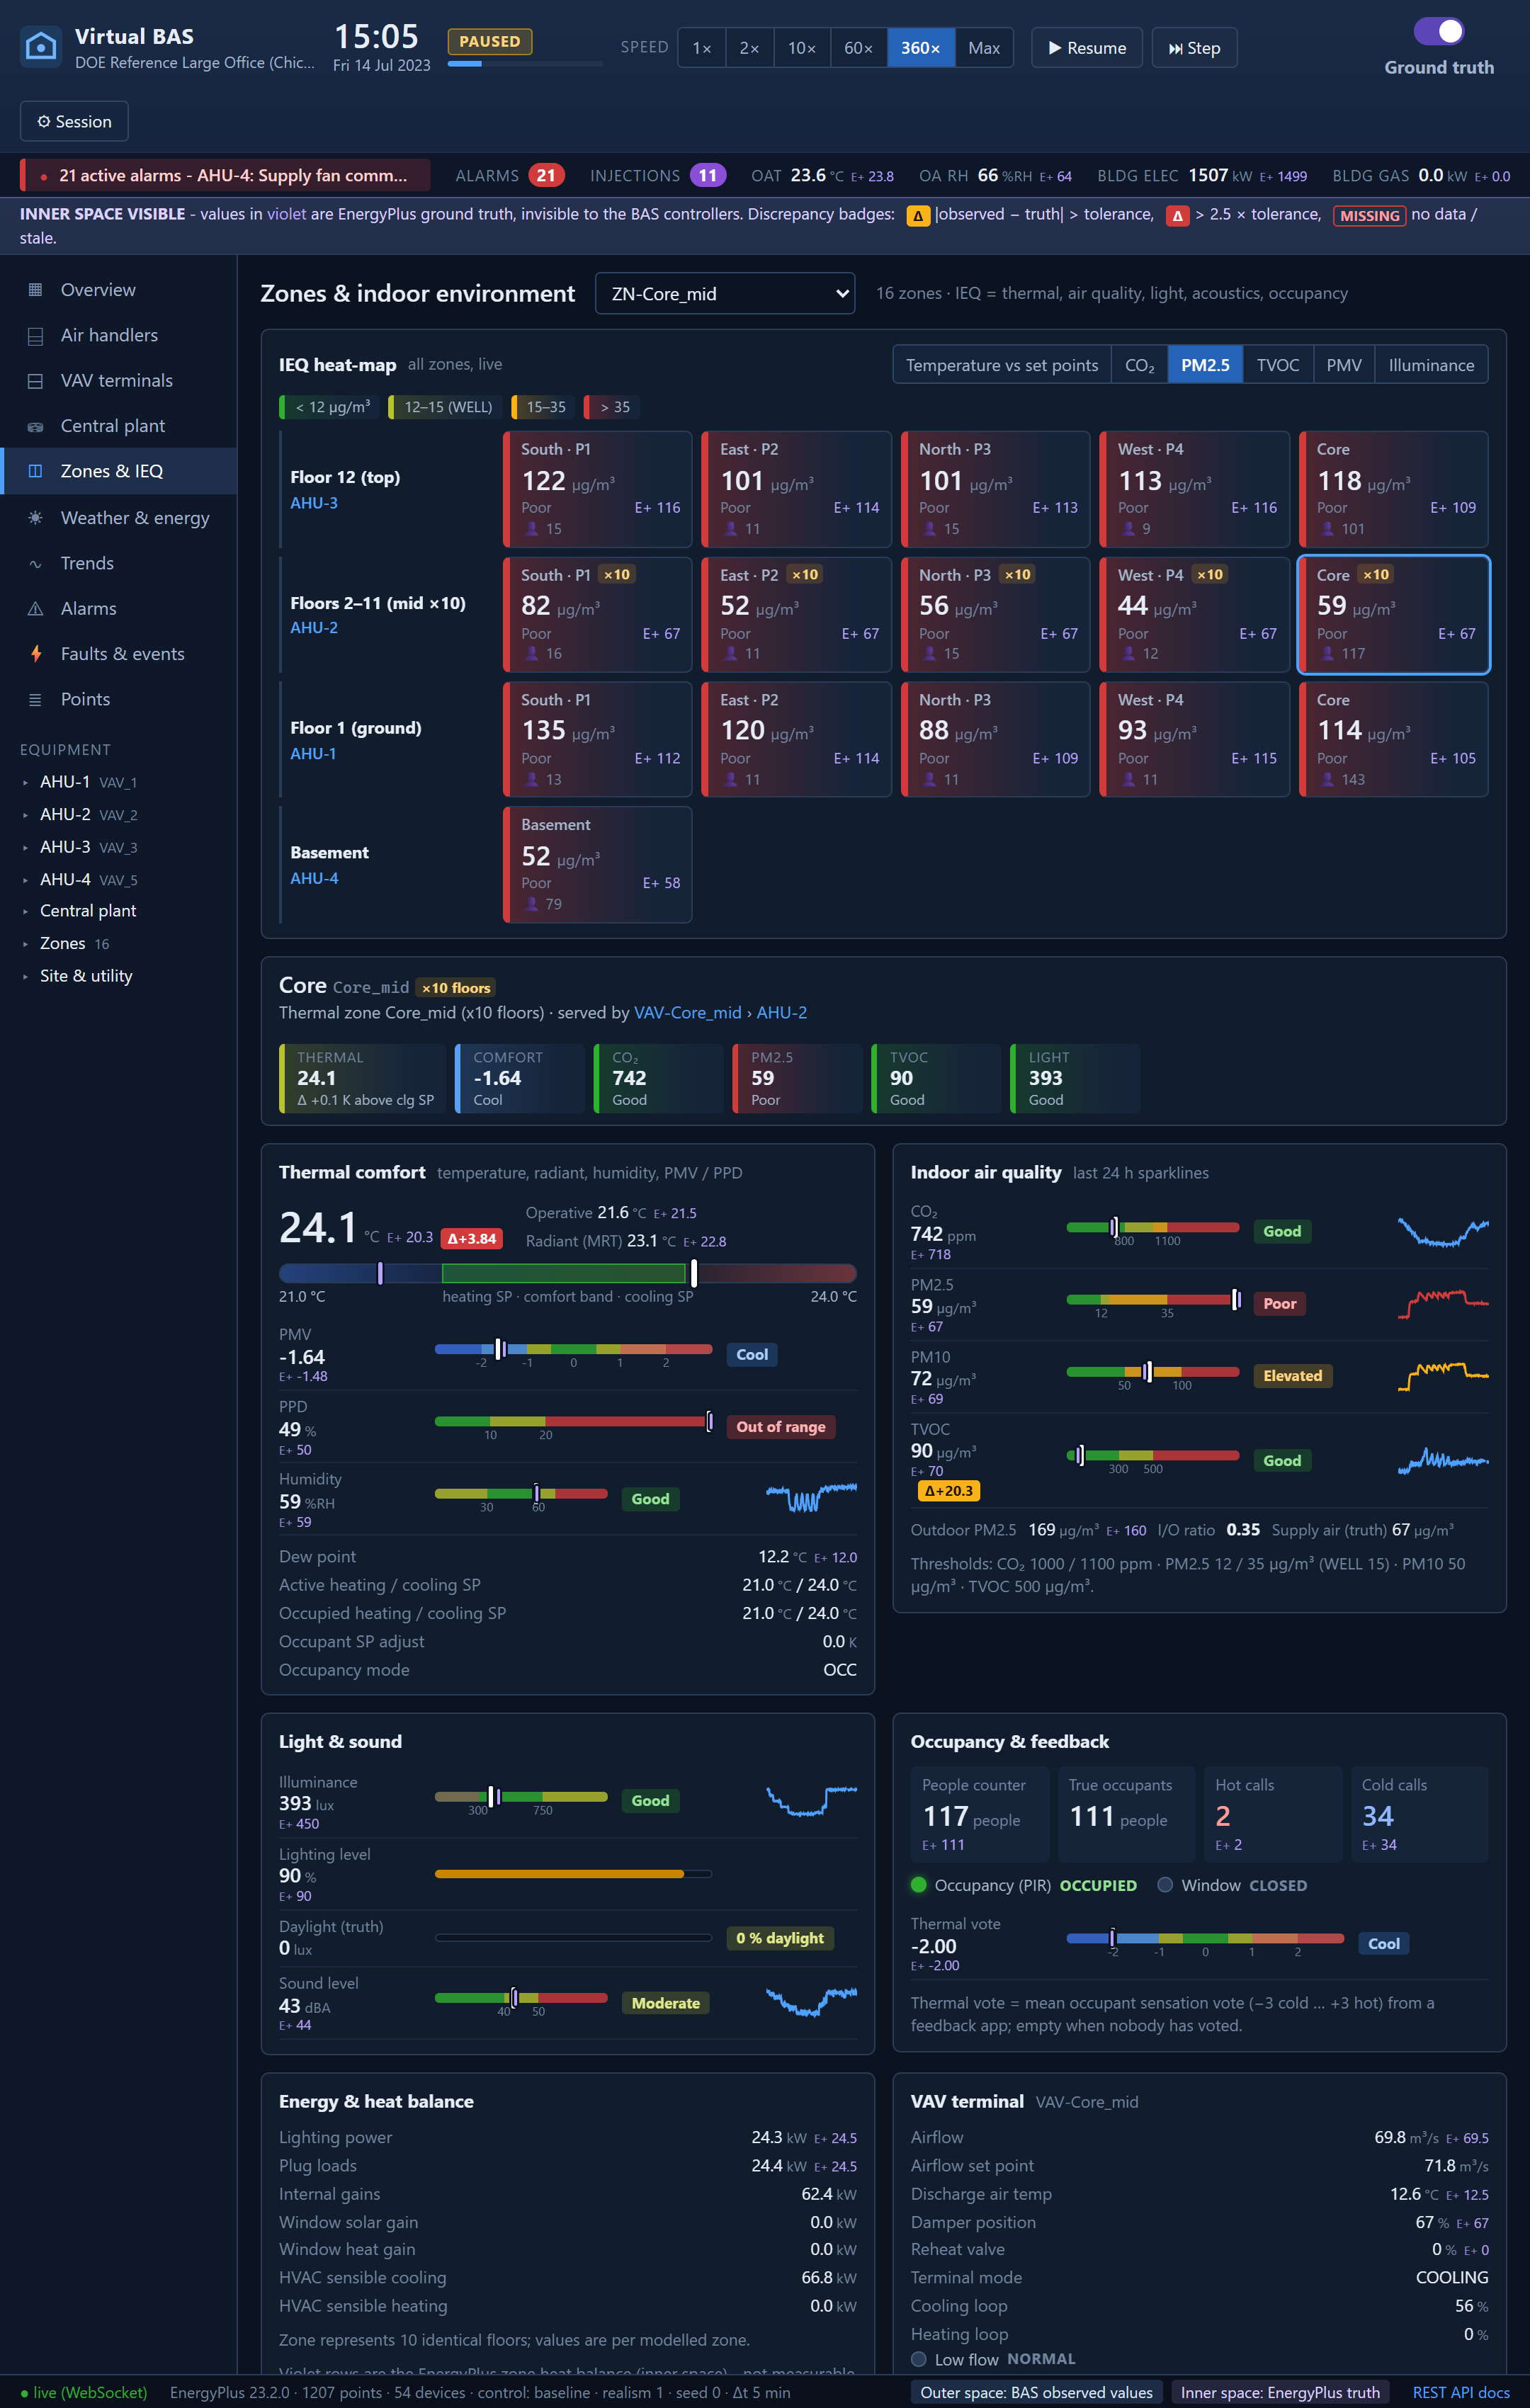
\includegraphics[width=0.49\textwidth]{gui_zone.png}\hfill
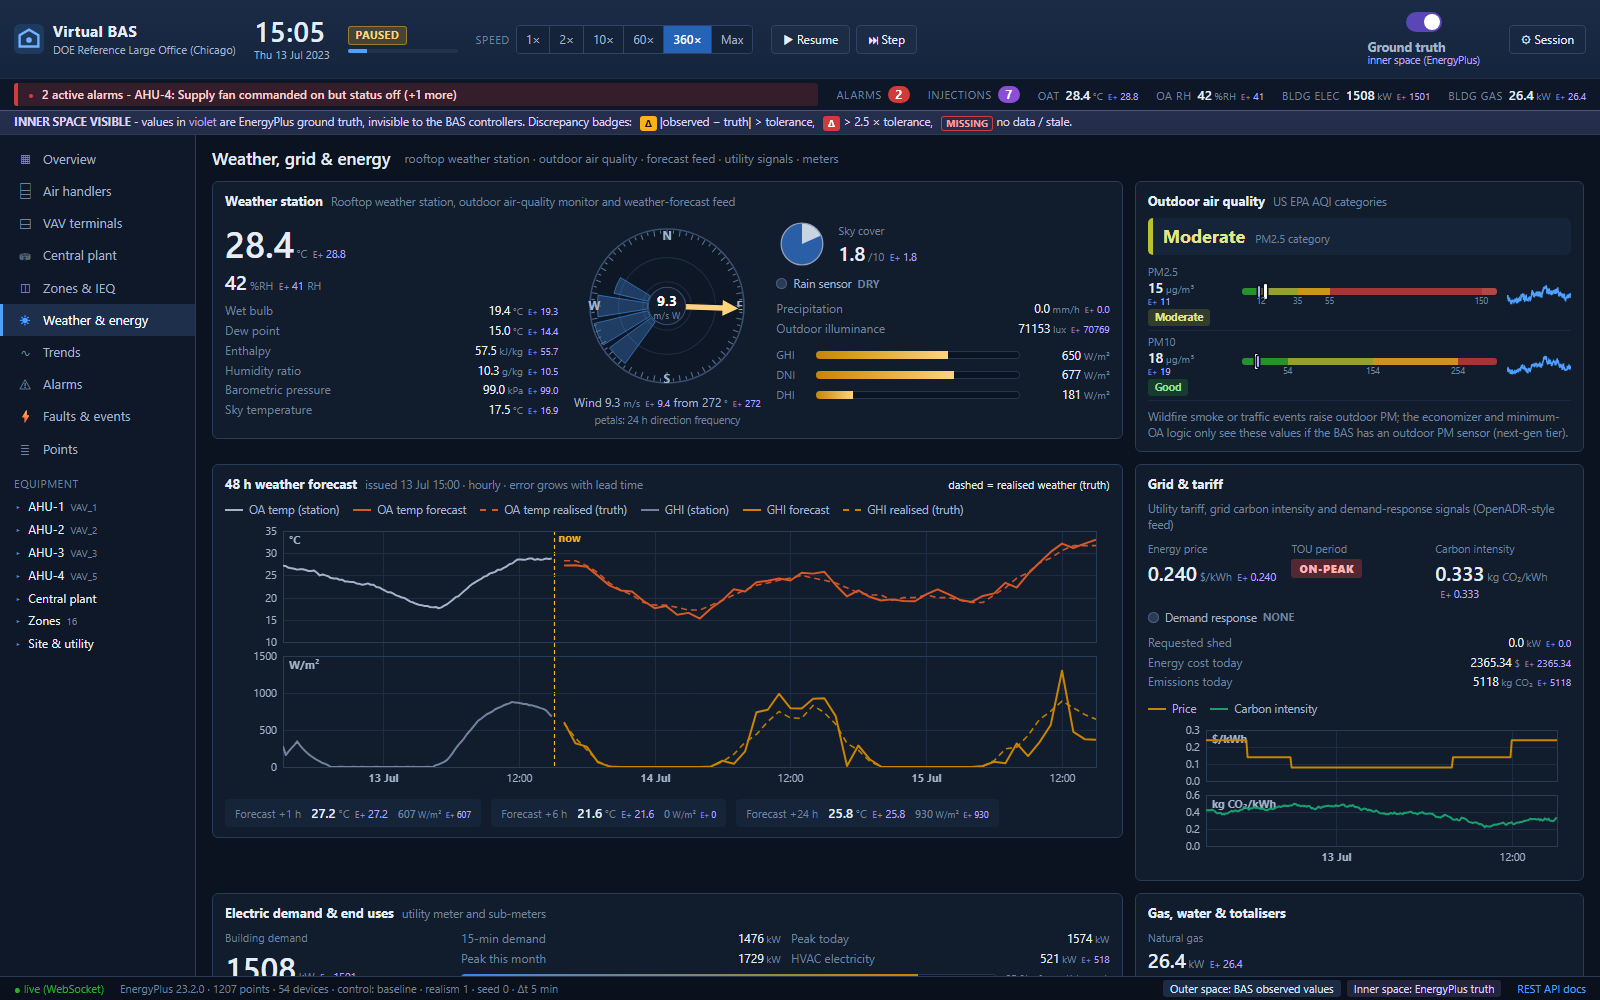
\includegraphics[width=0.49\textwidth]{gui_weather.png}
\caption{Web GUI of Virtual BAS with the ground-truth layer switched on: building overview (top left), AHU graphic
(top right), VAV box with a drifting zone sensor (observed vs. EnergyPlus truth badge, middle left), fault and event
injection console (middle right), zone indoor-environment page with a building heat-map (bottom left) and weather,
forecast, grid and energy page (bottom right).}
\label{fig:gui}
\end{figure*}

%==========================================================================================
\section{Case study}
\label{sec:case}

The DOE commercial reference large office (new construction, ASHRAE 90.1-2004, Chicago) \cite{deru2011reference}
distributed with EnergyPlus 23.2 is used. The 12-storey, \num{46320}~m$^2$ building is modelled with 19 zones
(basement, ground, a middle floor representing ten floors through a zone multiplier, and top floor, each with four
perimeter and one core zone, plus plenums), four VAV air handling units with economizers, chilled- and hot-water coils
and variable-speed fans, 16 VAV boxes with hot-water reheat, two water-cooled chillers, a cooling tower, a gas boiler
and three pumps. BAS-ization with a 5-min sampling interval yields \NumPoints{} points on \NumEquip{} pieces of
equipment (\NumSensorPts{} sensor and meter points, \NumSoftPts{} software points and \NumTruthPts{} ground-truth-only
points); \NumStdPts{} points are in the standard tier, \NumAdvPts{} advanced and \NumNextPts{} next-generation, and
\NumModelPts{} take their truth from outer-space or surrogate models. The model has 28 command schedules and 4
physical fault hooks. The Chicago TMY3 weather file is used and all runs use the
calendar year 2023. Experiments were run on a Windows 11 laptop with EnergyPlus 23.2 and Python 3.12.

%==========================================================================================
\section{Experiments and results}
\label{sec:results}

\subsection{Experiment 1: verification against native EnergyPlus}

The emulator must not distort the physics. A full year was simulated (i) natively in EnergyPlus with the original
controls and (ii) with Virtual BAS using ideal sensors (realism 0), deterministic occupancy and the baseline control
profile, with identical time step. Table~\ref{tab:validation} and Fig.~\ref{fig:validation} compare hourly results.
Annual whole-building electricity agrees within \ValElecDiffAbs\% (hourly CV(RMSE) \ValElecCV\%), cooling electricity
within \ValClgDiffAbs\% and fan electricity within \ValFanDiffAbs\%; natural gas is \ValGasDiff\% higher. The zone
temperatures of the 16 zones differ by \ValZoneMAE{}~K on average (MAE of hourly means). Lighting and plug loads are
identical by construction. Whole-building electricity and gas both satisfy the ASHRAE Guideline 14 hourly
calibration criteria (NMBE $\pm$10\%, CV(RMSE) 30\%) \cite{ashrae2014g14}; pump energy shows larger deviations. These
residual differences are expected and have a clear origin: the native model uses ideal controllers solved within
EnergyPlus' HVAC iterations, whereas the BAS controllers are sampled-data controllers acting every 5 min on values of
the previous sample. The largest differences occur at morning start-up, when the economizer and the preheat coil
interact during the first samples, and in pump energy, which reacts to short chilled-water demand events. Simulating a
year took \ValWallVBAS~s with Virtual BAS (105{,}120 BAS samples of \NumSensorPts{} sensor points, about
\ValStepsPerSec{} samples per second) versus \ValWallNative~s for the native batch simulation.

\begin{table}[!htbp]
\centering\small
\caption{Experiment 1: annual energy of native EnergyPlus and Virtual BAS (ideal sensors, baseline profile).}
\label{tab:validation}
\resizebox{\linewidth}{!}{\begin{tabular}{lrrrr}
\toprule
End use & Native [MWh] & Virtual BAS [MWh] & Diff. [\%] & CV(RMSE)$_h$ [\%] \\
\midrule
Electricity, total & 5,729 & 5,756 & +0.5 & 2.8 \\
Natural gas, total & 1,580 & 1,663 & +5.2 & 15.0 \\
Cooling (chillers) & 509 & 502 & -1.3 & 13.9 \\
Fans & 178 & 178 & +0.2 & 5.8 \\
Pumps & 258 & 295 & +14.1 & 44.4 \\
Heat rejection & 139 & 136 & -2.3 & 20.7 \\
Heating (boiler) & 1,511 & 1,594 & +5.5 & 15.7 \\
Interior lighting & 1,566 & 1,566 & +0.0 & 0.0 \\
Interior equipment & 2,329 & 2,329 & +0.0 & 0.0 \\
\midrule
Zone temp. MAE / RMSE [K] & \multicolumn{4}{l}{0.029 / 0.091 (mean of 16 zones)} \\
\bottomrule
\end{tabular}}
\end{table}

\begin{figure*}[t]
\centering
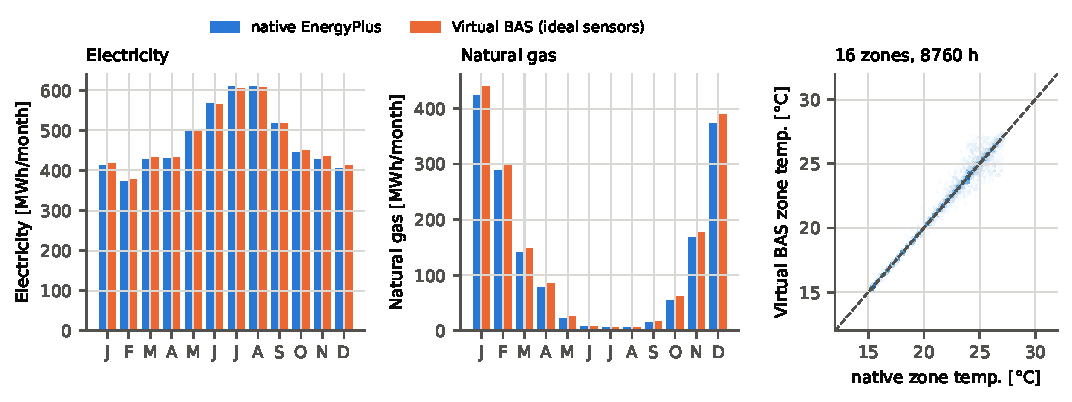
\includegraphics[width=\textwidth]{fig_validation.pdf}
\caption{Experiment 1: monthly electricity and natural gas (left, centre) and hourly zone temperatures of all 16
zones (right) of native EnergyPlus and Virtual BAS with ideal sensors.}
\label{fig:validation}
\end{figure*}

\subsection{Experiment 2: inner/outer-space coupling under sensor drift}

The motivating example was simulated for one summer week with realistic sensors and stochastic occupancy: the zone
temperature sensor of the core zone of the middle floors (representing ten floors) drifts by $+0.5$~K/day from the
second day, compared with a fault-free twin run with identical random streams (Fig.~\ref{fig:drift}). The VAV
controller keeps the \emph{observed} temperature at the cooling set point throughout. The \emph{true} temperature,
however, decreases day by day; at the end of the week the sensor reads \DriftErr~K above the truth. The controller
compensates the apparent overheating with more air: the mean discharge air flow during occupied hours increases by
\DriftFlow\%, and the building's HVAC electricity increases by \DriftHVAC\%. None of this is visible to a BAS operator
looking at the zone temperature trend. The run demonstrates the central mechanism of Virtual BAS: an outer-space
imperfection produces a wrong control signal, the wrong signal changes the physics, and the change is labelled.

\begin{figure*}[t]
\centering
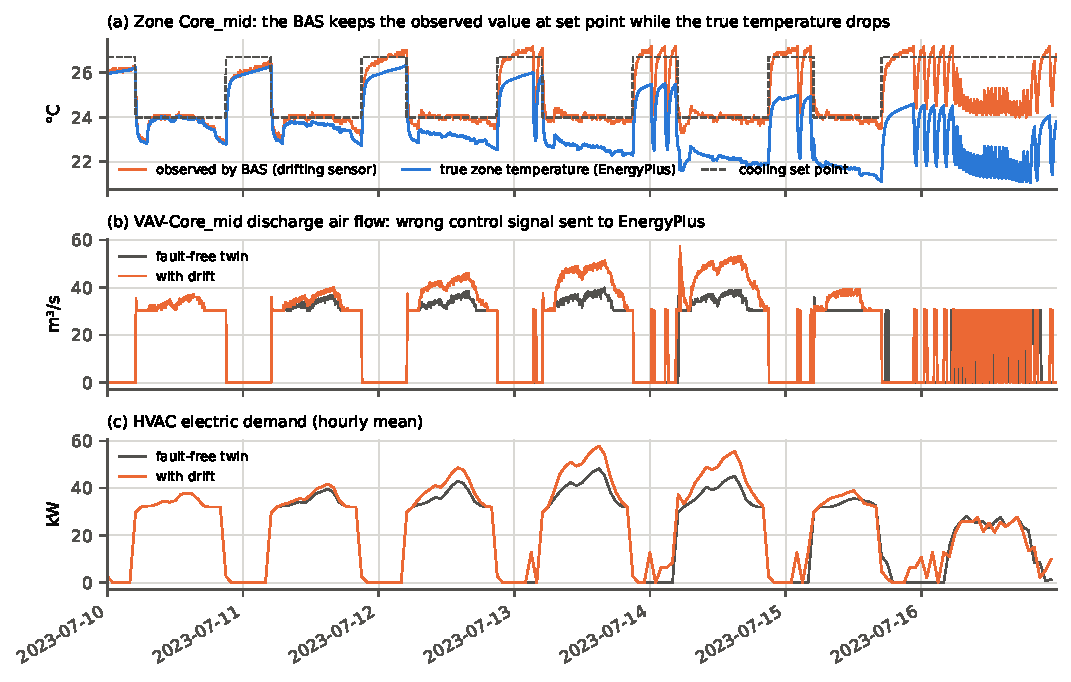
\includegraphics[width=\textwidth]{fig_drift_case.pdf}
\caption{Experiment 2: drift of the zone temperature sensor of zone Core\_mid. (a) Observed and true zone temperature;
(b) discharge air flow of the VAV box with and without drift; (c) HVAC electric demand.}
\label{fig:drift}
\end{figure*}

\begin{figure}[!htbp]
\centering
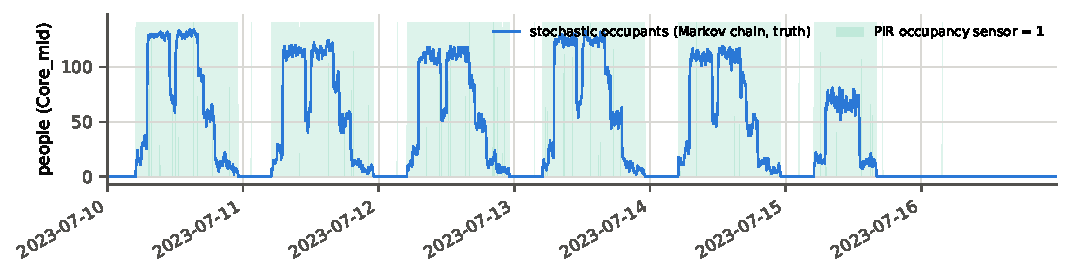
\includegraphics[width=\linewidth]{fig_occupancy.pdf}
\caption{Stochastic occupancy of zone Core\_mid (truth, written to EnergyPlus) and the corresponding PIR occupancy
sensor seen by the BAS during one summer week.}
\label{fig:occupancy}
\end{figure}

\subsection{Experiment 3: equipment-level fault impact matrix}

Twenty-seven single-fault scenarios covering all layers were each simulated for a summer and a winter week with
realistic sensors and stochastic occupancy and compared with the fault-free twin (common random numbers).
Fig.~\ref{fig:faultmatrix} reports the changes in electricity, gas and discomfort (occupied K$\cdot$h outside the
set-point band $\pm0.5$~K, computed from the truth); rows are grouped by layer (sensor, actuator, equipment, control,
network, events). The matrix shows physically consistent, season-dependent behaviour
at equipment level. A stuck-open outdoor-air damper of the main AHU increases winter gas by \FMoaGasW\% but has little
effect in summer; a closed damper saves heating energy at the cost of ventilation. A leaking reheat valve increases
summer gas consumption \FMleakGasS-fold relative to the fault-free week and causes \FMleakComfS~K$\cdot$h of
overheating. A stuck-closed chilled-water valve of AHU-1 produces \FMchwComfS~K$\cdot$h of summer discomfort but no
winter effect; a stuck-closed reheat valve does the opposite (\FMrhComfW~K$\cdot$h in winter). Chiller and tower fouling
raise summer electricity by \FMchFoulS\% and \FMtwFoulS\%, boiler fouling raises winter gas by \FMblFoulW\%, filter
fouling and fan degradation raise fan energy. A trip of one of the two chillers \emph{reduces} summer electricity because
the remaining chiller operates at a more efficient part-load ratio, while discomfort increases at peak load---a reminder
that fault impacts are not always energy penalties. A 24/7 schedule error on the main AHU increases summer electricity by
\FMschedS\%. Several faults are \emph{silent} in one season (e.g. economizer and mixed-air sensor faults in summer,
stuck-closed reheat valve in summer), an important property of real fault data that a dataset generator must
reproduce: labels mark fault presence, while the twin comparison quantifies fault impact.

\begin{figure}[!htbp]
\centering
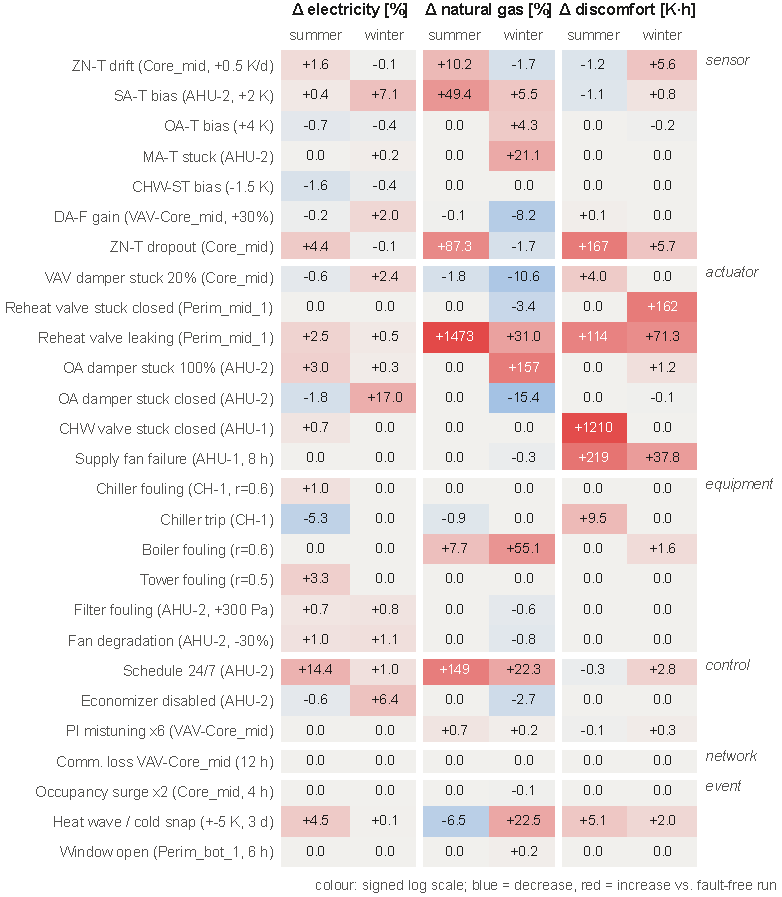
\includegraphics[width=\linewidth]{fig_fault_matrix.pdf}
\caption{Experiment 3: change of electricity, natural gas and discomfort relative to the fault-free twin for 27
single-fault scenarios (one week each, summer and winter). Colour: signed logarithmic scale.}
\label{fig:faultmatrix}
\end{figure}

\subsection{Experiment 4: labelled data generation and an FDD benchmark}

Two independent datasets were generated with the random fault generator restricted to nine AHU-level fault types
(sensor bias, drift and stuck on AHU temperature sensors, stuck outdoor-air damper, stuck-closed chilled-water valve,
filter fouling, fan degradation, disabled economizer, schedule error) at $\lambda=3$ per week: a training set
(April--June) and a test set (July--August) with different seeds. Hourly features (means and standard deviations of 23
quantities, e.g. supply-air temperature error, mixing-equation residual, outdoor-air damper command/feedback deviation,
fan power per flow, filter pressure drop) were computed from the \emph{observed} trend logs only, and labels from the
injection severity tables. A random forest \cite{breiman2001rf,pedregosa2011sklearn} trained on \FddTrainN{} AHU-hours
reaches a detection macro-F1 of \FddDetF{} and a diagnosis macro-F1 of \FddDiagF{} on \FddTestN{} test AHU-hours
(Fig.~\ref{fig:fdd}). The difficulty is genuine and informative: the test period lies in a different season, background
sensor errors and missing data are present, and several faults are unobservable under the prevailing conditions
(e.g. a disabled economizer in hot weather). The experiment demonstrates that Virtual BAS produces ML-ready,
consistently labelled data with controllable difficulty, distribution shift and realistic class imbalance.

\begin{figure}[!htbp]
\centering
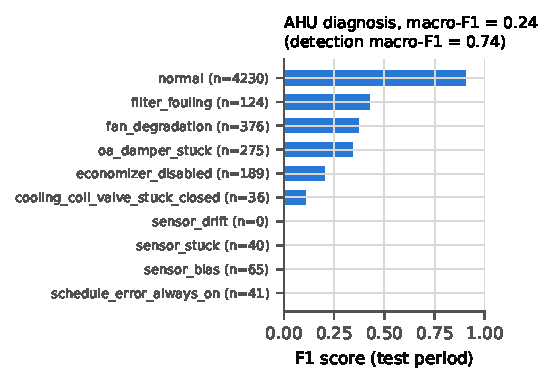
\includegraphics[width=0.8\linewidth]{fig_fdd.pdf}
\caption{Experiment 4: per-class F1 score of the AHU fault diagnosis benchmark on the test period.}
\label{fig:fdd}
\end{figure}

\subsection{Experiment 5: AI agents in the loop}

\paragraph{AI fault injection through the public API} An autonomous adversarial agent operated the building for six
days through the REST API, in lock-step with the simulation (pause, 6~h steps). Every six simulated hours it read the
BAS like an operator and chose an injection: forcing 100\% outdoor air on the AHU with the largest fan power when the
outdoor air was hot, an after-hours schedule error in the evening, and otherwise a slow drift of a zone thermostat. It
injected \AiInj{} faults, all recorded with \texttt{source=ai} and the agent's rationale. The same calls are exposed as
MCP tools, so an LLM agent can play the same role, for example to stress-test an FDD system.

\paragraph{Robustness of a supervisory AI controller} A supervisory agent resetting the AHU supply-air and
chilled-water set points from the observed outdoor-air temperature was evaluated through the Gymnasium interface in
three outer spaces---ideal sensors, realistic sensors, and realistic sensors with a $+4$~K bias of the outdoor-air
sensor---for two weeks in the shoulder season and in summer, each against the baseline BAS program in the same outer
space (Fig.~\ref{fig:ai}). In the shoulder season the agent reduces electricity by \AiShIdeal\% with ideal sensors and
\AiShReal\% with realistic sensors, but only by \AiShBias\% when the outdoor-air sensor reads 4~K high, because the
biased reading shifts every reset decision. At the same time the warmer supply air increases preheat and reheat gas
use by \AiShGasReal~MWh in two weeks (realistic sensors), so that site energy changes by \AiShSiteReal\%; in summer
the electricity saving is small (\AiSuReal\%). An evaluation restricted to electricity and to ideal sensors would
therefore have overstated the value of this policy twice. Such trade-offs and their sensitivity to measurement errors
must be understood before an AI controller is deployed, and they cannot be studied in an idealised environment.

\begin{figure}[!htbp]
\centering
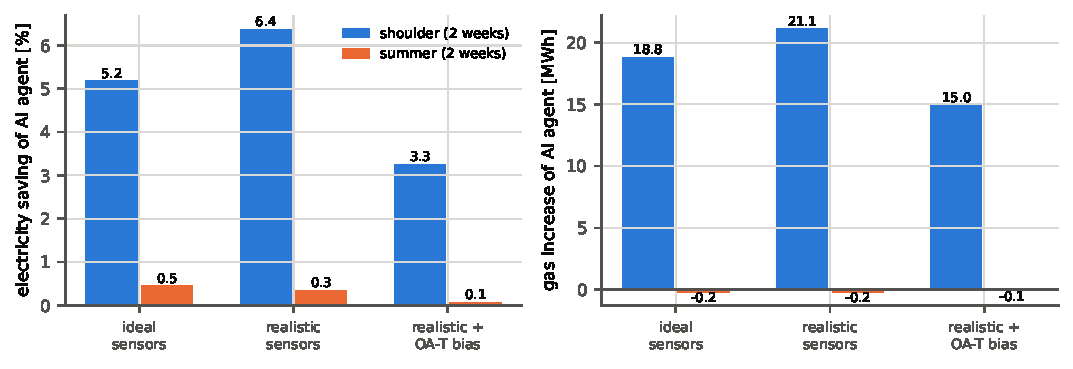
\includegraphics[width=\linewidth]{fig_ai_agent.pdf}
\caption{Experiment 5: electricity saving (left) and gas increase (right) of a supervisory AI controller relative to the
baseline BAS program in three outer spaces (ideal sensors, realistic sensors, realistic sensors with a $+4$~K
outdoor-air sensor bias).}
\label{fig:ai}
\end{figure}

\subsection{Experiment 6: indoor environment under wildfire smoke}

A summer week with a 30-h wildfire-smoke episode (outdoor PM2.5 up to \EnvPeakOut~$\mu$g/m$^3$) was simulated with
the reference MERV~8 filters, with MERV~13 filters, with a filter-bypass fault (60\% bypass, no pressure-drop symptom)
and with an IEQ-aware sequence that locks the economizers out while the outdoor PM2.5 exceeds 35~$\mu$g/m$^3$
(Fig.~\ref{fig:environment}a). Because the economizers bring up to 100\% outdoor air in this season, the mean indoor
concentration peaks at \EnvPeakEight~$\mu$g/m$^3$ with MERV~8, \EnvPeakBypass~$\mu$g/m$^3$ with the bypass fault,
\EnvPeakLock~$\mu$g/m$^3$ with the economizer lock-out and \EnvPeakThirteen~$\mu$g/m$^3$ with MERV~13; occupied
zone-hours above 35~$\mu$g/m$^3$ are \EnvHrsEight, \EnvHrsBypass, \EnvHrsLock{} and \EnvHrsThirteen. None of this is
visible in the standard tier: a typical BAS of today has no particle sensor, the bypass fault has no pressure-drop
symptom, and the lock-out decision requires the next-generation outdoor PM2.5 point. Figs.~\ref{fig:environment}b--d
show one day of the other environment points of a perimeter zone: illuminance with its daylight share and the
photosensor reading, TVOC flushed by the morning ventilation and its noisy metal-oxide reading, sound level, and PMV
with the sparse mean votes of the zone's occupants.

\begin{figure}[!htbp]
\centering
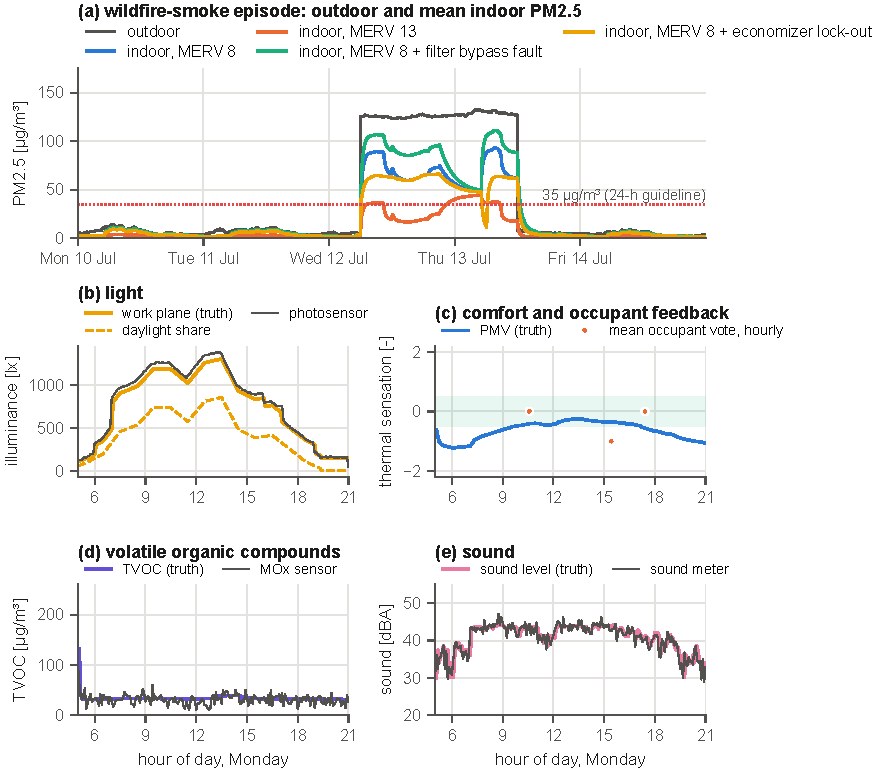
\includegraphics[width=\linewidth]{fig_environment.pdf}
\caption{Experiment 6: (a) outdoor and mean indoor PM2.5 during a wildfire-smoke episode for four filter/control
situations; (b)--(d) one summer day of illuminance, TVOC, sound and comfort points of a perimeter zone (truth and
sensor readings).}
\label{fig:environment}
\end{figure}

\subsection{Experiment 7: time acceleration}

The pacing accuracy was measured by setting target speed factors while running (Fig.~\ref{fig:speed}). The achieved
speed matches the target within \SpeedErr\% for factors from 10 to 3600; at maximum speed one BAS sample takes
\SpeedMs~ms, i.e. \SpeedMaxK{} times real time, so one simulated year runs in about \ValWallVBASmin{} minutes. Real time
(1$\times$) follows from the same pacing law. The speed can be changed, paused or single-stepped at any moment from the
GUI or the API, which allows the same environment to serve real-time interaction with people or deployed agents and
fast training of learning agents.

\begin{figure}[!htbp]
\centering
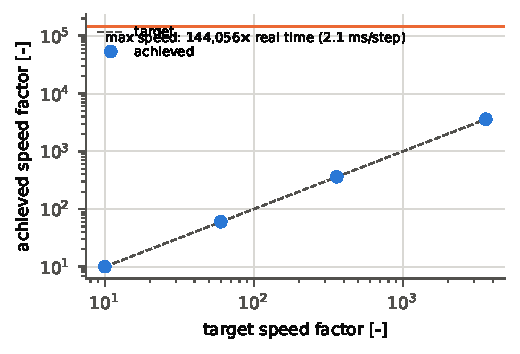
\includegraphics[width=0.75\linewidth]{fig_speed.pdf}
\caption{Experiment 7: target versus achieved speed factor and maximum throughput.}
\label{fig:speed}
\end{figure}

\subsection{Experiment 8: generality}

The BAS-ization procedure was applied without any building-specific code to five DOE reference buildings
(Table~\ref{tab:generality}). All models were converted and simulated for one week. Multi-zone VAV systems with
water-based plants (large office, hospital, secondary school) are fully BAS-controlled; the medium office (packaged VAV
with DX cooling and electric reheat) and the small office (packaged single-zone units) are monitored completely and
their terminals and thermostats are BAS-controlled while unsupported components keep their native local control. The
hospital, with 55 zones and four 100\%-outdoor-air and mixed-air AHUs, yields \NumHospitalPts{} points on 128 pieces of
equipment and runs at \HospitalSps{} samples per second.

\begin{table}[!htbp]
\centering\small
\caption{Experiment 8: automatic BAS-ization of five DOE reference buildings (one-week runs).}
\label{tab:generality}
\resizebox{\linewidth}{!}{\begin{tabular}{lrrrrrrr}
\toprule
Building & Zones & VAV & AHUs & Plant loops & Equipment & Points & Samples/s \\
\midrule
Large office & 16 & 16 & 4 & 4 & 48 & 518 & 185 \\
Medium office & 15 & 15 & 3 & 1 & 35 & 375 & 386 \\
Small office & 5 & 0 & 5 & 1 & 12 & 180 & 594 \\
Hospital & 55 & 55 & 4 & 4 & 125 & 1366 & 114 \\
Secondary school & 46 & 41 & 9 & 3 & 104 & 1207 & 106 \\
\bottomrule
\end{tabular}}
\end{table}

%==========================================================================================
\section{Discussion}
\label{sec:discussion}

\subsection{Potential uses and impact}
\label{sec:uses}

A real BAS is a poor place to learn, experiment or certify: faults cannot be staged on demand, the true state is
unknown, every mistake affects occupants and equipment, a year of operation takes a year, and access is restricted by
owners, vendors and cyber-security policies. Virtual BAS removes each of these barriers at once---it is safe to break,
labelled, repeatable through seeded scenarios, faster than real time, free and open, and it can be generated for any
EnergyPlus model. Table~\ref{tab:uses} lists eighteen uses that follow from these properties, grouped into four areas,
together with the users, the enabling features and the evidence available in this paper. The table distinguishes uses
that the experiments demonstrate from uses for which the interfaces exist but no evaluation is reported here.

\begin{table*}[p]
\centering
\caption{Potential uses of Virtual BAS, with primary users in italics. Evidence: Exp.~$n$ = demonstrated in
Experiment~$n$; \emph{interf.} = all required functions are implemented but not evaluated in this paper;
\emph{partial} = some functions are missing (see Section~\ref{sec:limitations}).}
\label{tab:uses}
\scriptsize
\renewcommand{\arraystretch}{1.08}
\begin{tabularx}{\textwidth}{@{}>{\raggedright\arraybackslash}p{50mm}>{\raggedright\arraybackslash}X>{\raggedright\arraybackslash}p{14mm}@{}}
\toprule
Use (\emph{users}) & What Virtual BAS provides & Evid. \\
\midrule
\multicolumn{3}{@{}l}{\textbf{Research and development of building AI}}\\
FDD development and benchmarking (\emph{FDD researchers, analytics developers}) & Unlimited labelled data with controlled fault type, severity, season and sensor quality; closed-loop tests & Exp.~3, 4 \\
Supervisory, MPC and RL control (\emph{control and RL researchers}) & Gymnasium; sensor errors, missing data and faults; ideal vs.\ realistic outer space on the same physics & Exp.~5 \\
Ambient-AI and LLM operators (\emph{AI researchers, BAS vendors}) & MCP tools, overrides and alarms at any speed; ground truth for scoring; agents as operators and adversaries & Exp.~5 \\
Foundation models (\emph{machine-learning researchers}) & Diverse, labelled, multivariate BAS time series for any EnergyPlus model \cite{emami2023buildingsbench} & Exp.~4, 8 \\
Virtual sensing and sensor recalibration (\emph{researchers}) & Observed and true values side by side; defined bias, drift, lag and data-loss models & Exp.~2 \\
Metadata inference, portable apps (\emph{researchers, integrators}) & Haystack/Brick point lists with known metadata for converted buildings \cite{gao2015metadata} & Exp.~8 \\
Value of information, sensor design (\emph{sensor makers, standard writers}) & Standard, advanced and next-generation tiers; one scenario seen through different instrumentation & Exp.~6 \\
\multicolumn{3}{@{}l}{\textbf{Education and workforce development}}\\
University courses (\emph{instructors, students}) & BAS-like GUI; equipment that can be broken safely; truth switch; open scenarios; a season in one lab session & interf. \\
Operator and facility-manager training (\emph{owners, utilities, training programmes}) & Drills with hidden or random faults; alarms, trends and overrides as in a real BAS; labels as answer key & interf. \\
Commissioning practice (\emph{commissioning agents}) & Functional tests of sequences, staged faults, trend review against known causes & interf. \\
Emergency and resilience drills (\emph{facility managers}) & Wildfire smoke, heat waves, cold snaps, equipment trips, demand response at run time & Exp.~6 \\
Alarm management, HMI research (\emph{human-factors researchers}) & Reproducible alarm floods and faults for user studies under identical conditions \cite{isa182} & interf. \\
\multicolumn{3}{@{}l}{\textbf{Industry practice}}\\
Testing commercial FDD and analytics (\emph{owners, efficiency programmes}) & Blind test buildings with known faults and severities; scoring against labels & Exp.~4 \\
Sequence verification, virtual commissioning (\emph{designers, contractors}) & G36-style sequences in closed loop and under sensor faults before site work \cite{wetter2022obc} & Exp.~2, 3 \\
BAS and analytics software (\emph{vendors, start-ups}) & A mock building behind REST, WebSocket and MCP for integration tests and demonstrations & interf. \\
Cyber-physical security (\emph{security researchers}) & Spoofed readings, malicious overrides, controller and historian outages, physical impact \cite{granzer2010security} & partial \\
Grid-interactive buildings (\emph{utilities, aggregators}) & Tariff, carbon intensity, demand-response events, demand meters \cite{neukomm2019geb} & interf. \\
\multicolumn{3}{@{}l}{\textbf{Research community}}\\
Benchmarks, competitions, reproducibility (\emph{all}) & Seeded scenarios, open building models, common KPIs, public code & Exp.~1--8 \\
\bottomrule
\end{tabularx}
\end{table*}

\paragraph{Research and development of building AI} Virtual BAS is first a proving ground for building AI. FDD
developers obtain unlimited labelled data with controllable fault rates, severities, seasons and sensor quality and
can test algorithms in closed loop (Experiments~3 and 4). Control and RL researchers can evaluate policies under partial
observability, sensor errors, missing data and equipment faults, and quantify robustness by switching the outer space
while keeping the inner space fixed (Experiment~5). Ambient-AI and LLM agents can be connected through MCP and
evaluated on operational tasks (diagnosing complaints, finding faults, writing safe overrides) with exact ground
truth; they can also act as adversaries that generate challenging scenarios. Because any EnergyPlus model can be
converted, the emulator can also produce the large and diverse corpora of BAS-level, multivariate, labelled time
series that foundation models for building operation will need; existing synthetic corpora for pre-training cover
whole-building loads only \cite{emami2023buildingsbench}. The point tiers support sensor-placement and
value-of-information studies: the same scenario can be observed through the instrumentation of a typical BAS and
through next-generation sensing, and the benefit of, e.g., coil energy meters, people counters or particle monitors for
a given task can be measured against ground truth (Experiment~6).

\paragraph{Education and workforce development} Students rarely get write access to a real BAS, and when they do they
cannot break it. With Virtual BAS a course on HVAC systems, controls or building data science can let every student
operate the same building, change set points and sequences, inject a stuck damper or a drifting sensor and see both
what the BAS shows and what really happens; time acceleration fits a season of operation into a laboratory session.
For operators, facility managers and technicians the same features become troubleshooting drills. The GUI hides the
ground truth by default, an instructor injects faults from the console or lets the random fault generator choose them,
the trainee works only with graphics, trends, alarms and overrides, and the label record then serves as the answer key
for scoring. This brings to building operation the simulator-based training that is standard in aviation and nuclear
power \cite{ans35} and has so far been limited to prototypes in buildings \cite{xu2004training,johra2020geenie}.
Commissioning agents can rehearse functional tests, and facility managers can practise responses to wildfire smoke,
heat waves, equipment trips and demand-response events. Reproducible alarm floods also make it possible to study
alarm management and operator interfaces with human participants \cite{isa182}.

\paragraph{Industry practice} Owners and efficiency programmes that procure FDD or analytics services currently have no
neutral way to compare products; a blind Virtual BAS building with known faults gives such a test, scored against the
labels (Experiment~4). Designers and control contractors can exercise sequences in closed loop, including their
behaviour under sensor faults, before the site work, complementing formal specification and verification workflows
\cite{wetter2022obc}. BAS and analytics vendors obtain a mock building for continuous integration, demonstrations and
training of their own staff. Security researchers can emulate spoofed readings with sensor-layer faults, malicious
commands with overrides and outages with network-layer faults, and observe the physical impact of an attack
\cite{granzer2010security}. Utilities and aggregators can test demand-response and carbon-aware strategies with the
tariff, grid and demand-meter points \cite{neukomm2019geb}. Given the savings at stake in commissioning
\cite{mills2011commissioning} and controls \cite{fernandez2017controls}, even a modest improvement in how people and
software operate buildings has a large aggregate effect.

\paragraph{Research community} Seeded scenarios, open building models and common KPIs allow benchmarks and competitions
in which every participant faces the same faults, sensor errors and occupants, and allow results to be reproduced
exactly. This addresses a recurrent obstacle of FDD and building-AI research, in which methods are evaluated on
private data that others cannot access \cite{katipamula2005review1,kim2018fddreview}.

\subsection{Limitations and future work}
\label{sec:limitations}

\paragraph{Limitations} (i) Local loops inside EnergyPlus are ideal; set-point translation reproduces their steady
state under sensor error but not their fast dynamics, hunting or valve characteristics. (ii) Duct static and loop
differential pressures are surrogate models because EnergyPlus does not resolve pressure networks. (iii) The 5-min
sampling interval limits the dynamics of BAS loops; finer intervals are possible at proportionally higher cost.
(iv) Explicit BAS control currently covers multi-zone VAV systems with water-based plants; other system types are
monitored and keep native control. (v) Fault parameters follow data-sheet-type distributions rather than calibrated
field statistics; the framework accepts any distribution. (vi) The verification shows residual differences of a few
percent in gas and pump energy caused by sampled-data versus ideal control. (vii) The environment does not yet speak
building network protocols. (viii) The extended environment models (well-mixed zones, lumen and daylight-flux
methods, fan-law acoustics, stochastic feedback, synthetic grid signals) and the refrigerant, flue and vibration
surrogates are simplified and not calibrated against measurements; the filter pressure drop does not yet depend on
the MERV class, and ozone, NO$_2$, formaldehyde, glare and envelope heat flux are not modelled. The tier assignment
reflects guideline point lists and field surveys and will differ between buildings.

\paragraph{Future work} A BACnet/IP and Modbus gateway so that commercial BAS front ends and analytics can connect
unchanged; Spawn-of-EnergyPlus or Modelica inner spaces for faster local dynamics; calibrated fault occurrence
statistics; multi-building portfolios; and standardised benchmark tasks for LLM-based building operators. For
education and training, an instructor/trainee mode that withholds labels and active injections from the trainee's
session and scores diagnoses automatically, together with course modules and drill libraries developed and evaluated
with instructors and building operators. For security studies, a dedicated library of cyber-attacks on BAS
protocols. The educational and training uses in Table~\ref{tab:uses} have not yet been evaluated with learners; such
studies are planned.

%==========================================================================================
\section{Conclusions}
\label{sec:conclusions}

This paper presented Virtual BAS, a real-world-like building automation system emulator that separates the physics
(EnergyPlus, inner space) from a mathematically defined and fully labelled real world (outer space). Sensors drift,
data go missing, occupants move randomly, equipment and control software fail, and the BAS acts on what it sees, so the
consequences of imperfection are simulated rather than superimposed. Faults and events can be injected at run time
by humans and AI agents, the clock runs from real time to more than \SpeedMaxK{} times real time, and any EnergyPlus
model can be converted. For the DOE large office, the emulator reproduces native EnergyPlus within \ValElecDiffAbs\%
in annual electricity with ideal sensors, produces physically consistent equipment-level fault signatures, generates
labelled datasets for FDD, supports AI agents as operators, controllers and adversaries, and exposes robustness gaps
that idealised environments hide. Beyond AI research, the same properties---safe to break, labelled, repeatable, fast
and open---make it a training simulator for students, operators, facility managers and commissioning agents, a neutral
test building for commercial FDD and analytics products, and a shared benchmark for the research community. The
software, building models, scenarios, experiments and tutorials are openly available to help the community develop
building AI, and the people who operate buildings, for real buildings.

%==========================================================================================
\section*{CRediT authorship contribution statement}
\textbf{Liang Zhang:} Conceptualization, Methodology, Software, Validation, Formal analysis, Investigation, Data
curation, Writing -- original draft, Writing -- review \& editing, Visualization, Project administration.

\section*{Declaration of competing interest}
The author declares that he has no known competing financial interests or personal relationships that could have
appeared to influence the work reported in this paper.

\section*{Data availability}
The software, the prepared building models, all scenarios, the experiment scripts and tutorials are openly available
at \url{https://github.com/TensorBuildLab/Virtual-BAS} under the MIT license. All results in this paper can be
regenerated with the scripts in the \texttt{experiments/} and \texttt{paper/} folders.

\section*{Declaration of generative AI and AI-assisted technologies in the manuscript preparation process}
During the preparation of this work the author used Claude (Anthropic) to assist with software implementation,
running the experiments and drafting the manuscript text. After using this tool, the author reviewed and edited the
content as needed and takes full responsibility for the content of the published article.

\bibliographystyle{elsarticle-num}
\bibliography{references}

\end{document}
